 % -*- root: ../main.tex -*-
\documentclass[../main.tex]{subfiles}
\begin{document}

\chapter{Caractérisation des interactions croisées entre hormones thyroïdiennes et glucocorticoïdes dans les bourgeons de membres postérieurs}


% -----------------------------------------
% --- BEGIN - Résumé

\section{L'interaction croisée des hormones thyroïdiennes et des glucocorticoïdes dans les pattes postérieures révèle une perturbation des programmes de mise en place du squelette}

	\subsection{Résumé et portée de l'article}\label{subsec:grimaldi2014}
	J'ai dans un premier temps consacré mes efforts à l'analyse des programmes transcriptionnels régulés par les \glspl{ht} et les \glspl{gc} dans les bourgeons de membres postérieurs de têtards de \gls{xtrop}.
	Ces organes sont au \gls{snf} 54 en plein développement, et font intervenir des processus cellulaires très variés, de la prolifération à l'apoptose.
	Ce modèle d'étude est particulièrement pertinent dans le cadre des impacts à long terme de perturbations survenant lors du développement post-embryonnaire.
	\par
	Comme décrit précédemment, l'analyse de la dynamique du transcriptome de cet organe après 24h de traitement aux \glspl{ht} et/ou aux \glspl{gc} est réalisée par \gls{rnaseq}.
	Le détail de la procédure utilisée au cours de cette partie de l'analyse est décrit dans la section ``Materials and Methods'' de la publication en cours de finition présentée à la \autoref{subsec:grimaldi2014}.
	\par
	Le résultat fort qui découle de ce travail concerne la fonction biologique des gènes dont l'expression induite ou réprimée par une des deux hormones est affectée par la seconde.
	Les profils d'expression peuvent ainsi être classifiés en deux catégories :
	``antagonistes'' quand l'effet de la première hormone est inhibée par la seconde ; ``potentiés'' dans le cas d'une additivité ou une synergie d'action entre les deux hormones.
	\par
	L'analyse préliminaire basée sur l'annotation fonctionnelle de ces gènes par \gls{go} révèle que seul un certain type de profil semble enrichi en une fonction biologique particulière (voir \autoref{par:hlc-go-pot-down}).
	Pour aller plus loin et se détacher des biais potentiel bien connus des bases de données d'annotation fonctionnelles (meilleure caractérisation dans un contexte mammalien, biais vers certaine fonctions biologiques ...), chaque gène dans les différentes catégories d'interactions croisées entre \gls{ht} et \gls{gc} a été annoté manuellement sur la base de la littérature.
	Il ressort de cette analyse qu'une part significative de ces gènes sont impliqués dans le remodelage de la matrice extra-cellulaire, du cartilage, et de l'os.
	Alors qu'il est bien décrit dans la littérature que les \glspl{ht} et les \glspl{gc} sont cruciaux lors du développement squelettique \citep{Robson2002,Wojcicka2013a}, ces données apportent les premiers éléments de réponse moléculaires vers une élucidation du rôle et des conséquences développementales de l'interaction croisée entre deux voies de signalisation.

	% --- END - Résumé article
	% -----------------------------------------

	% :::::::::::::::::::::::::::::::::::::::::

	% -----------------------------------------
	% --- BEGIN - Article

	% \iftoggle{deadtree}{
	% 	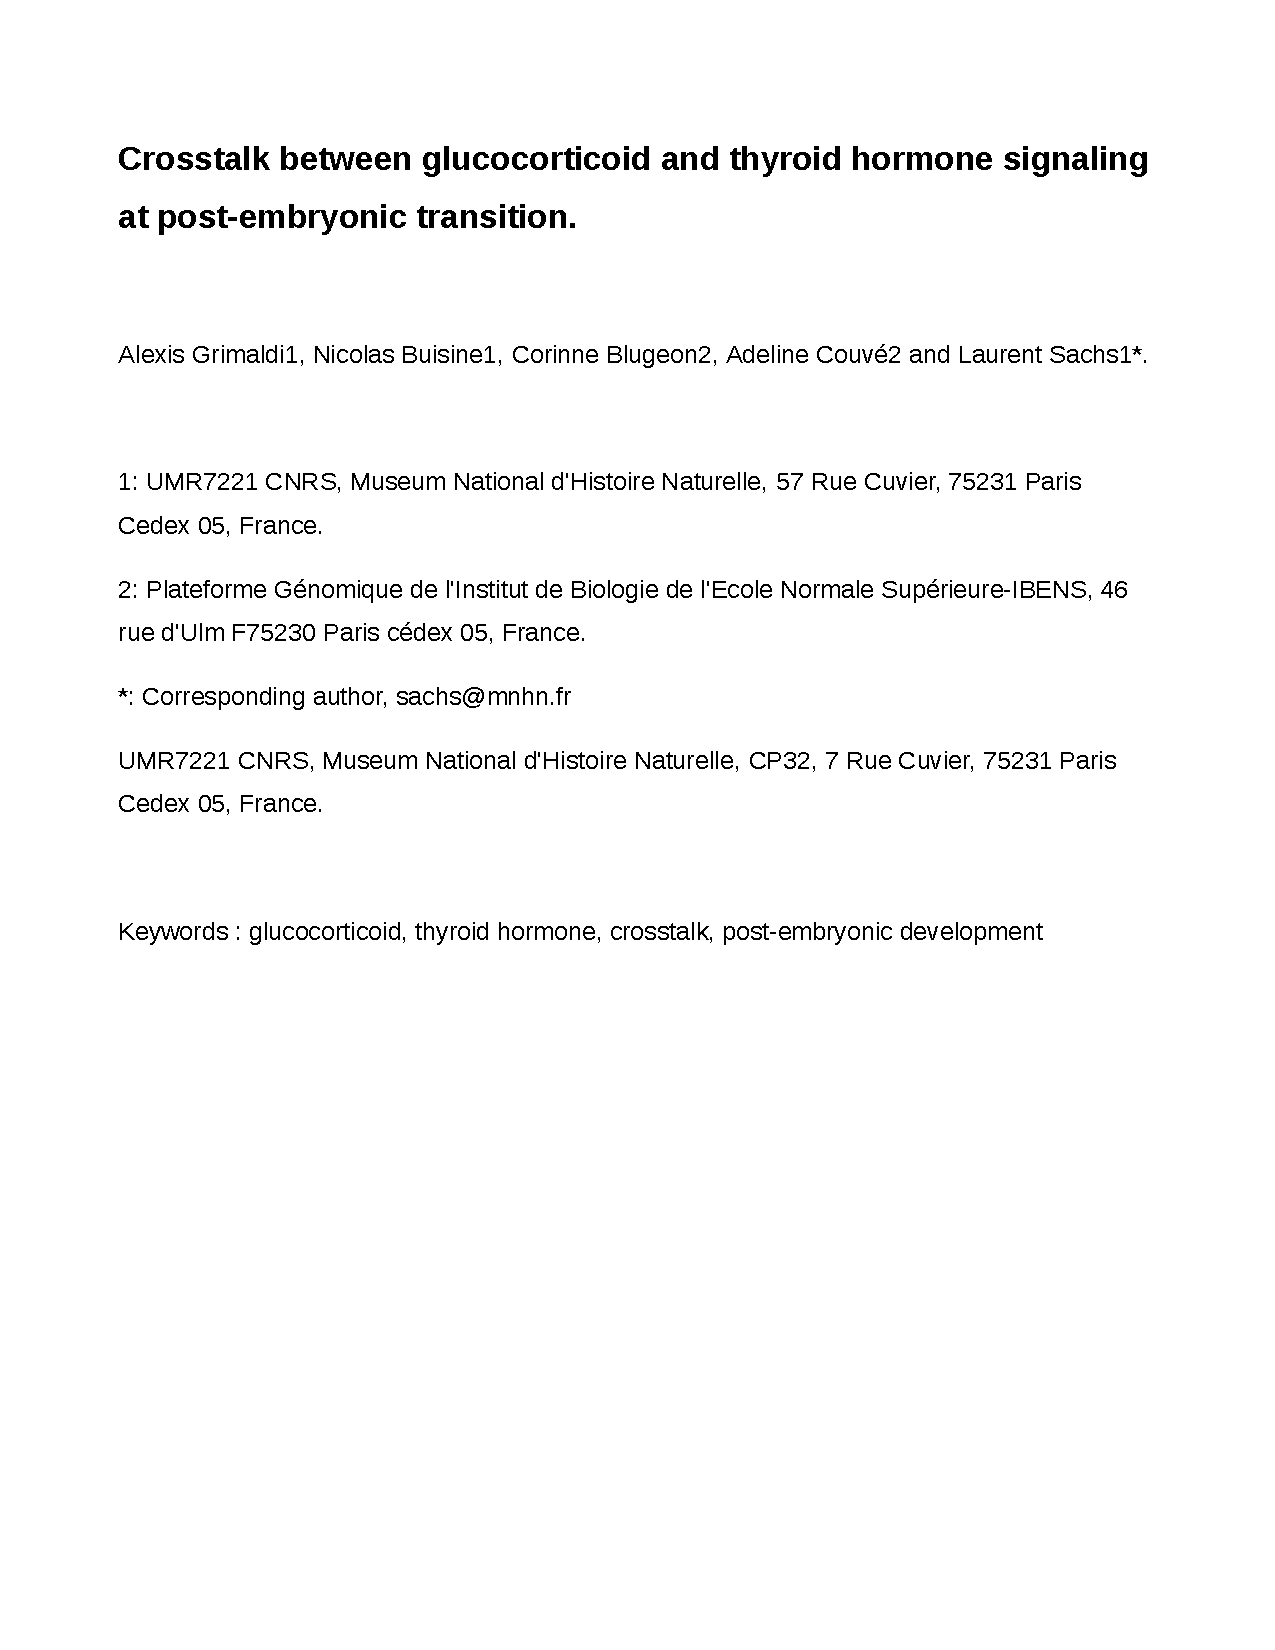
\includepdf[pages={-},nup=1x2,landscape=true]{Publications/grimaldi2014.pdf}
	% 	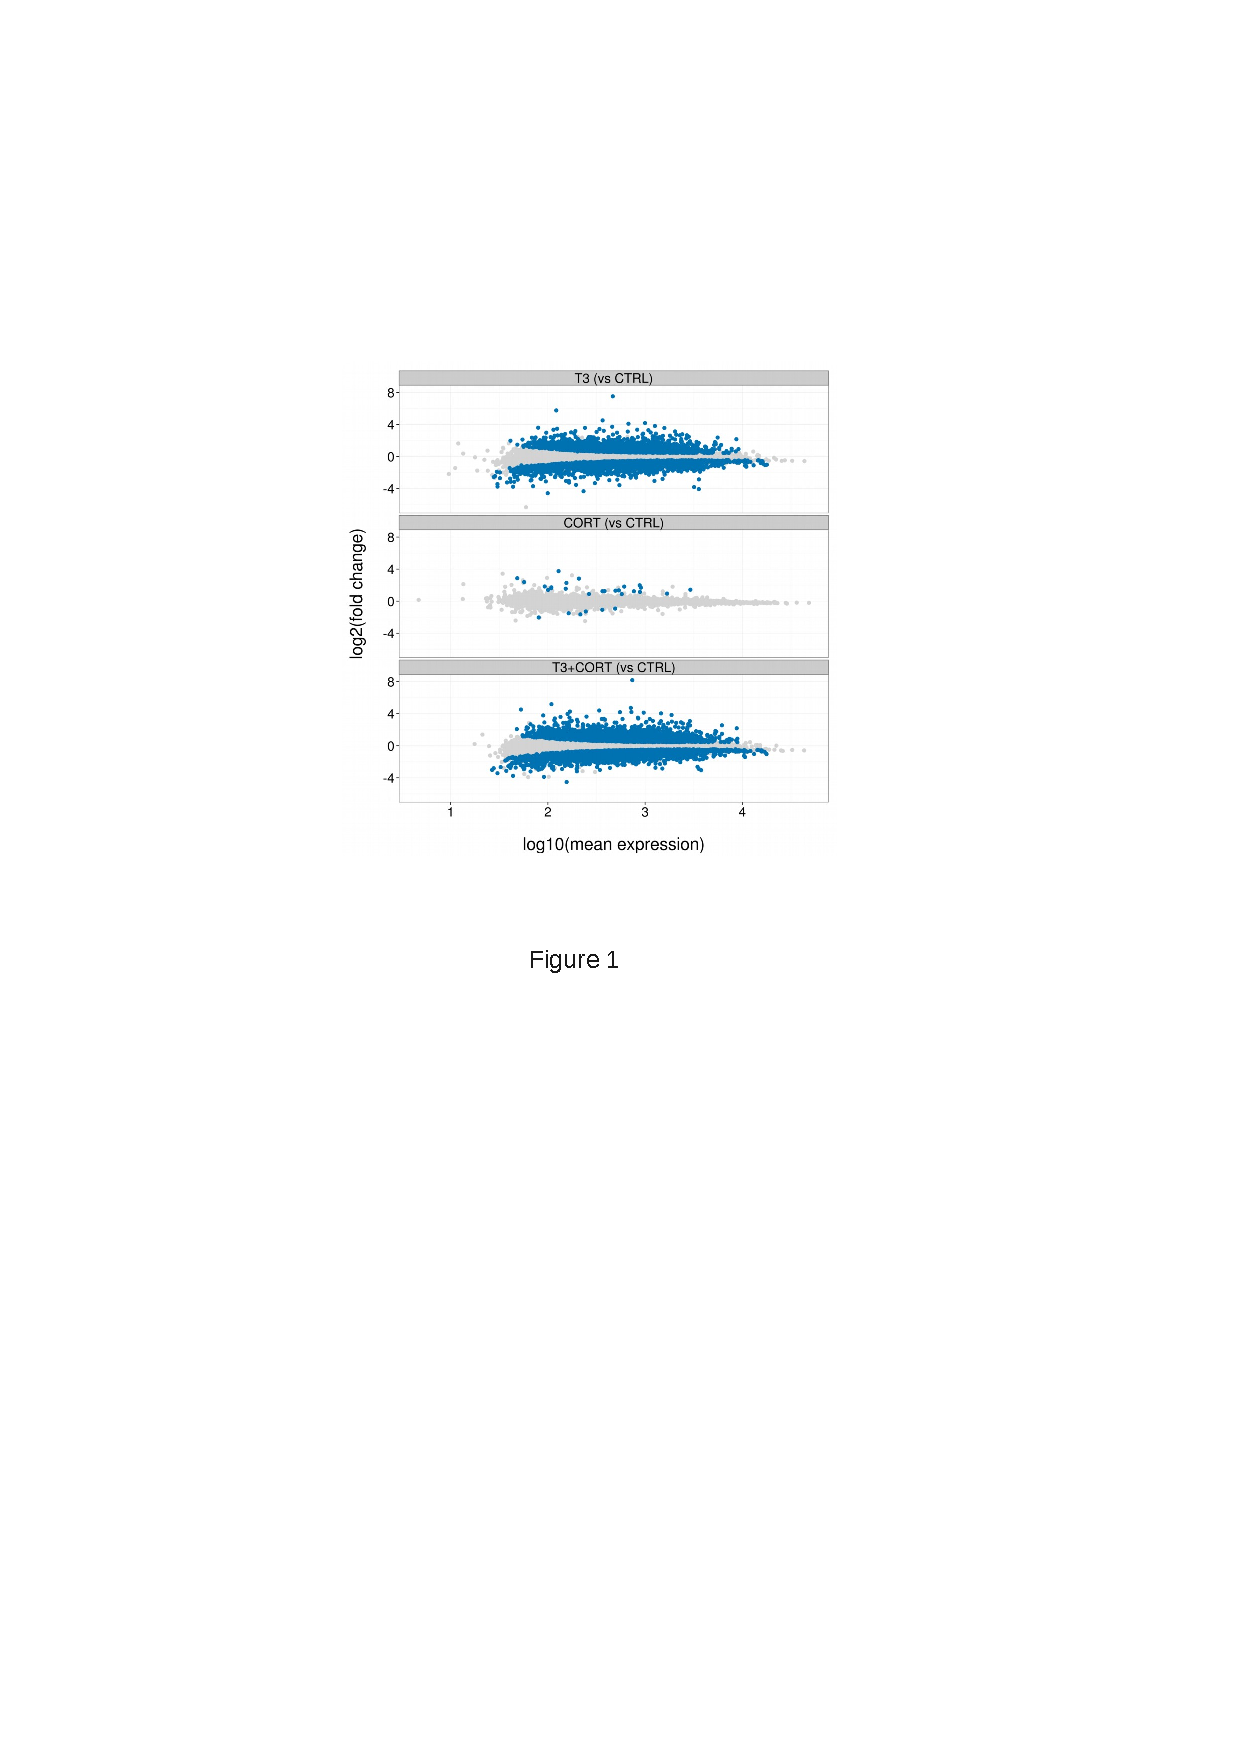
\includepdf[pages={-},nup=1x2,landscape=true]{Publications/grimaldi2014-fig.pdf}
	% 	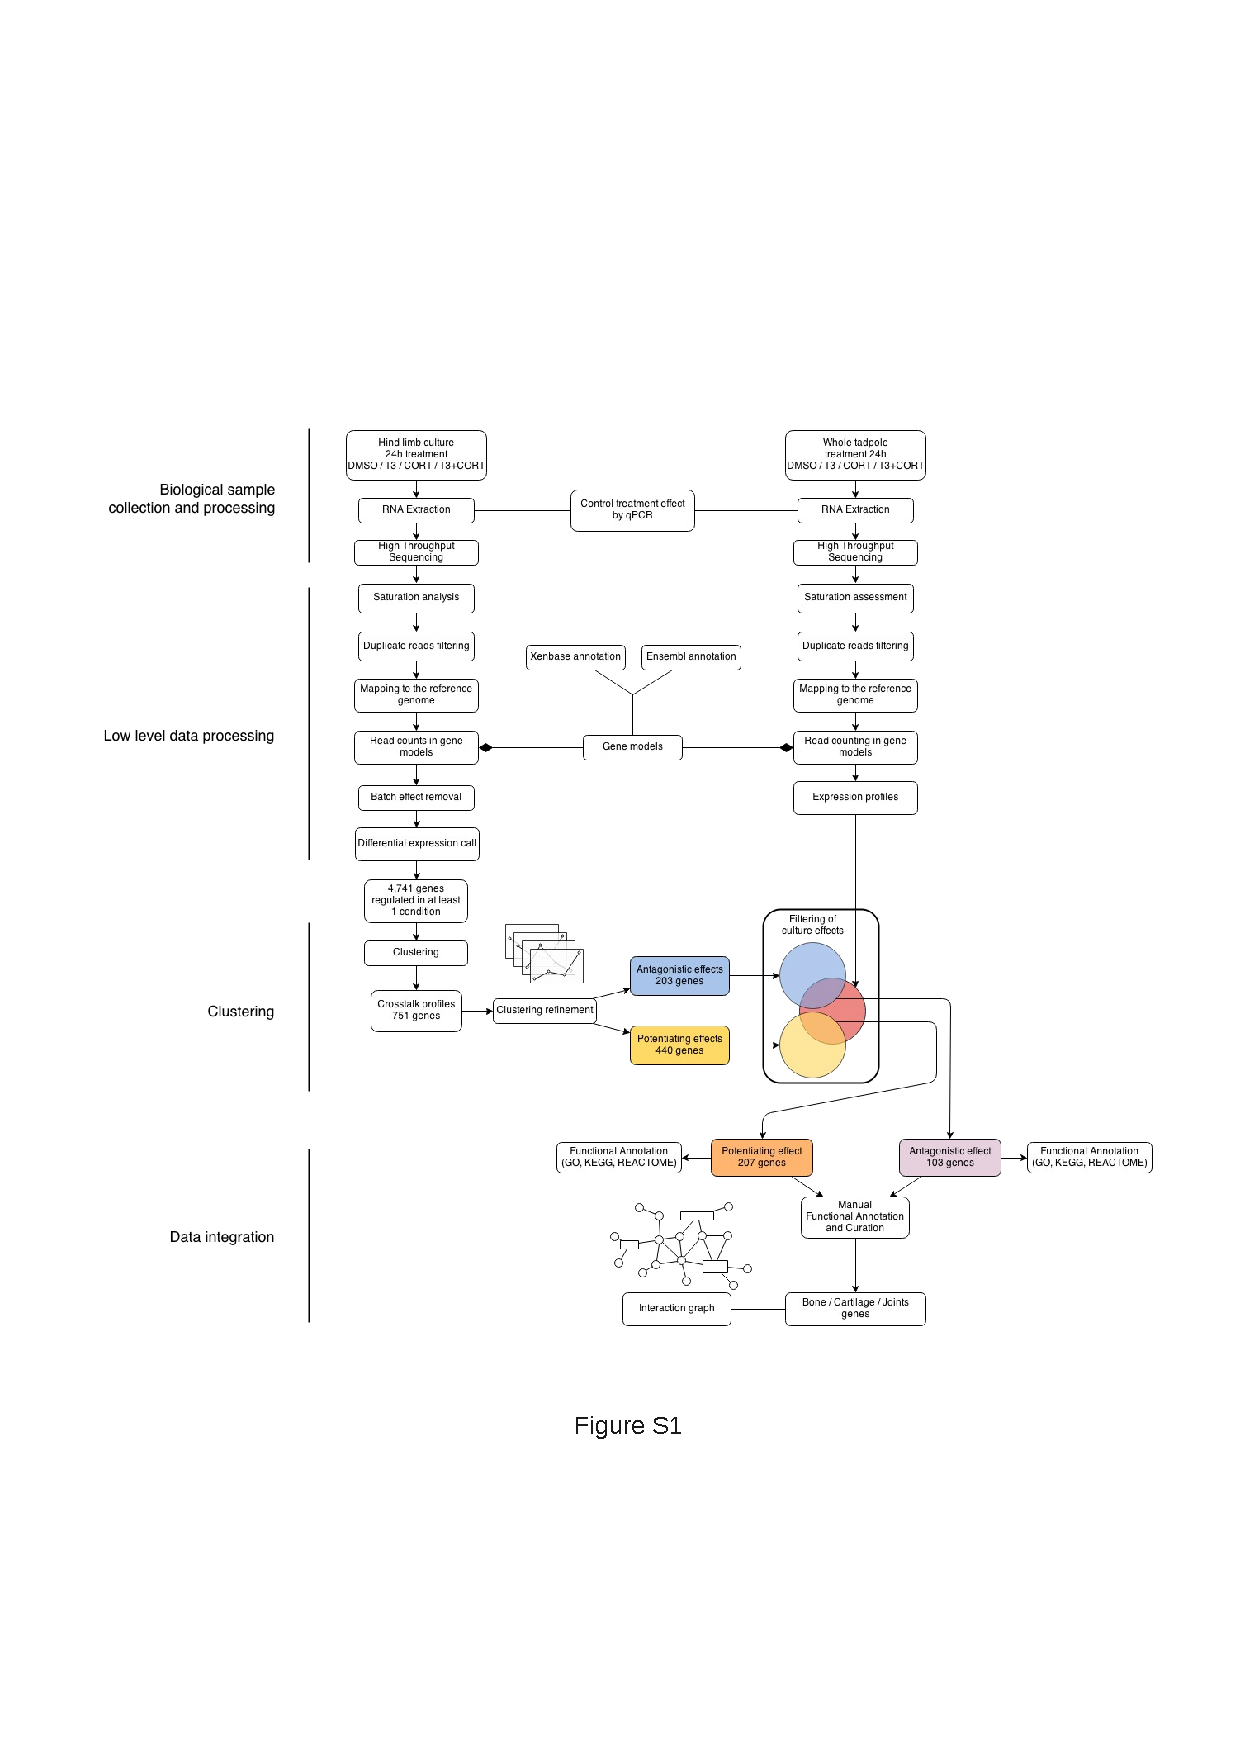
\includepdf[pages={-},nup=1x2,landscape=true]{Publications/grimaldi2014-sup.pdf}
	% }{
		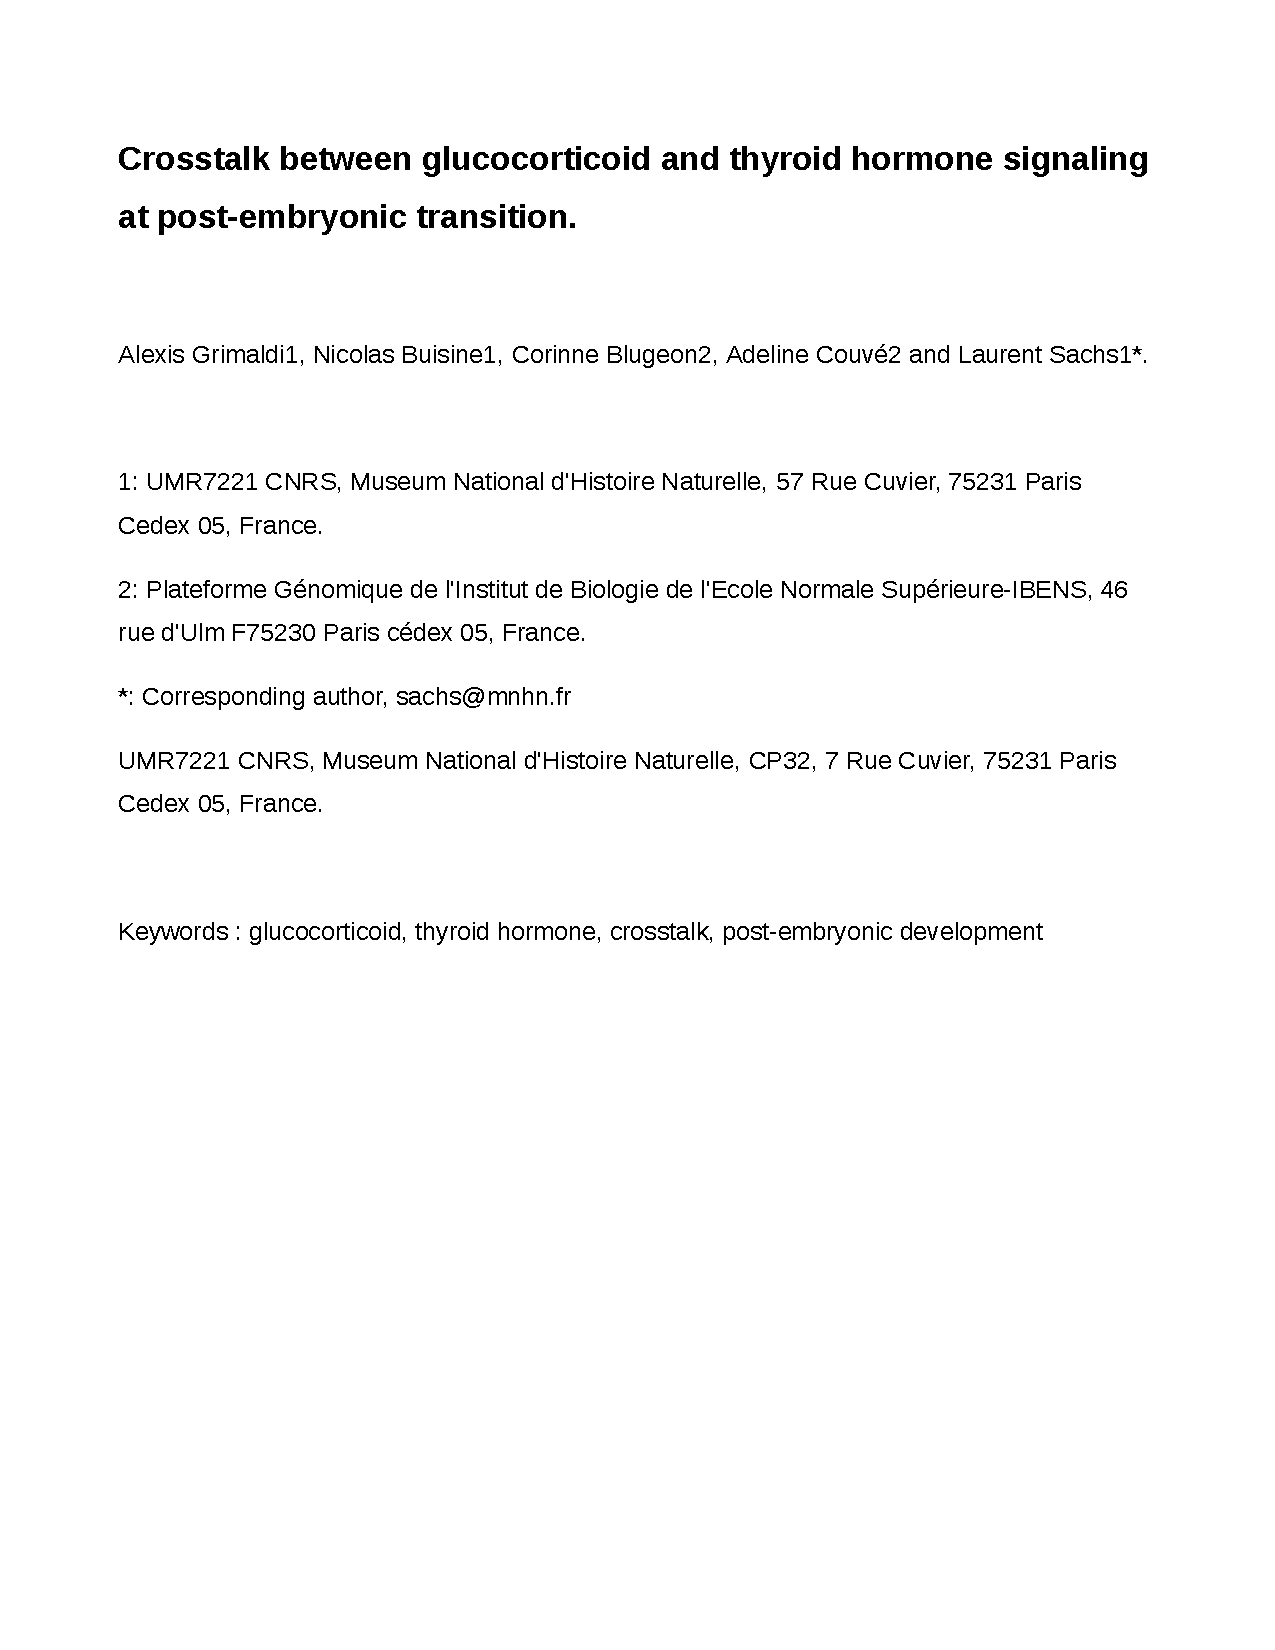
\includepdf[pages={-}]{Publications/grimaldi2014.pdf}
		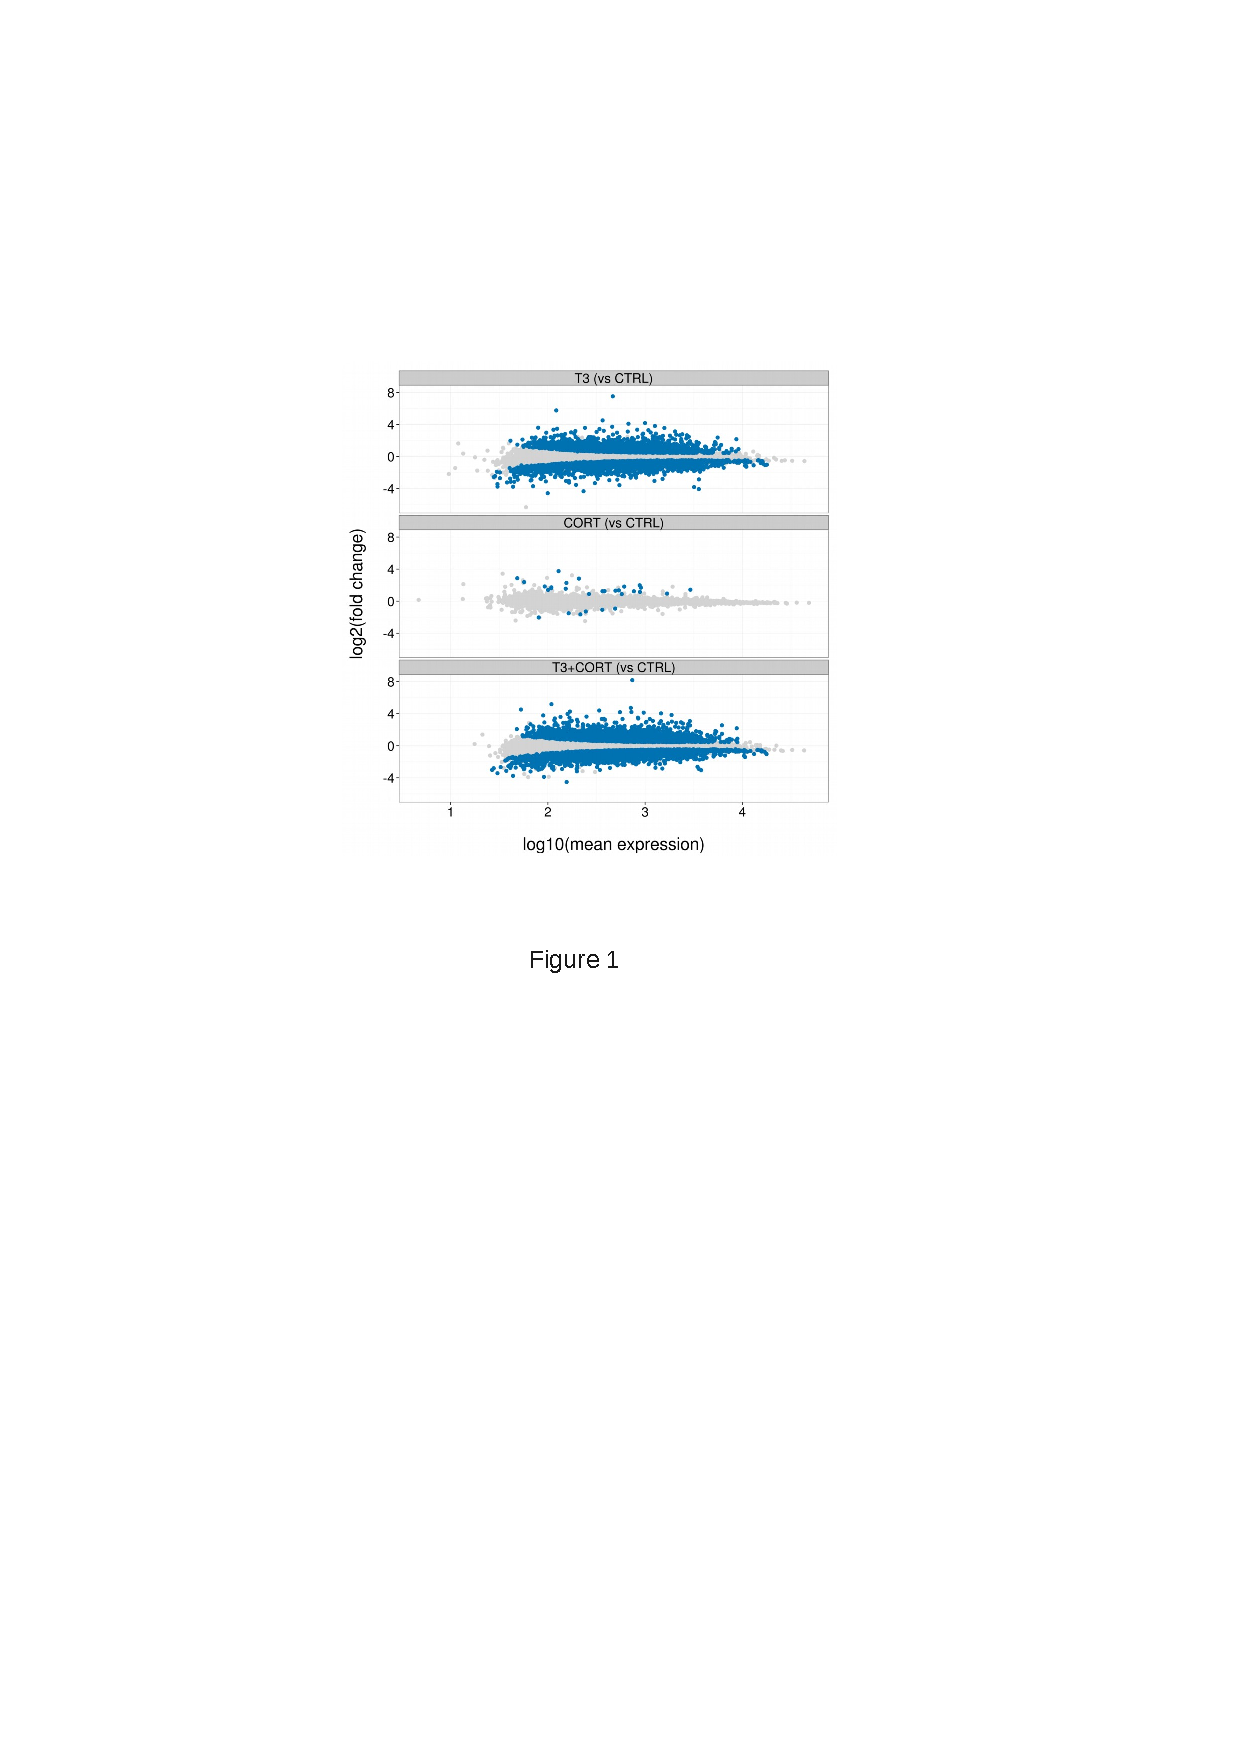
\includepdf[pages={-}]{Publications/grimaldi2014-fig.pdf}
		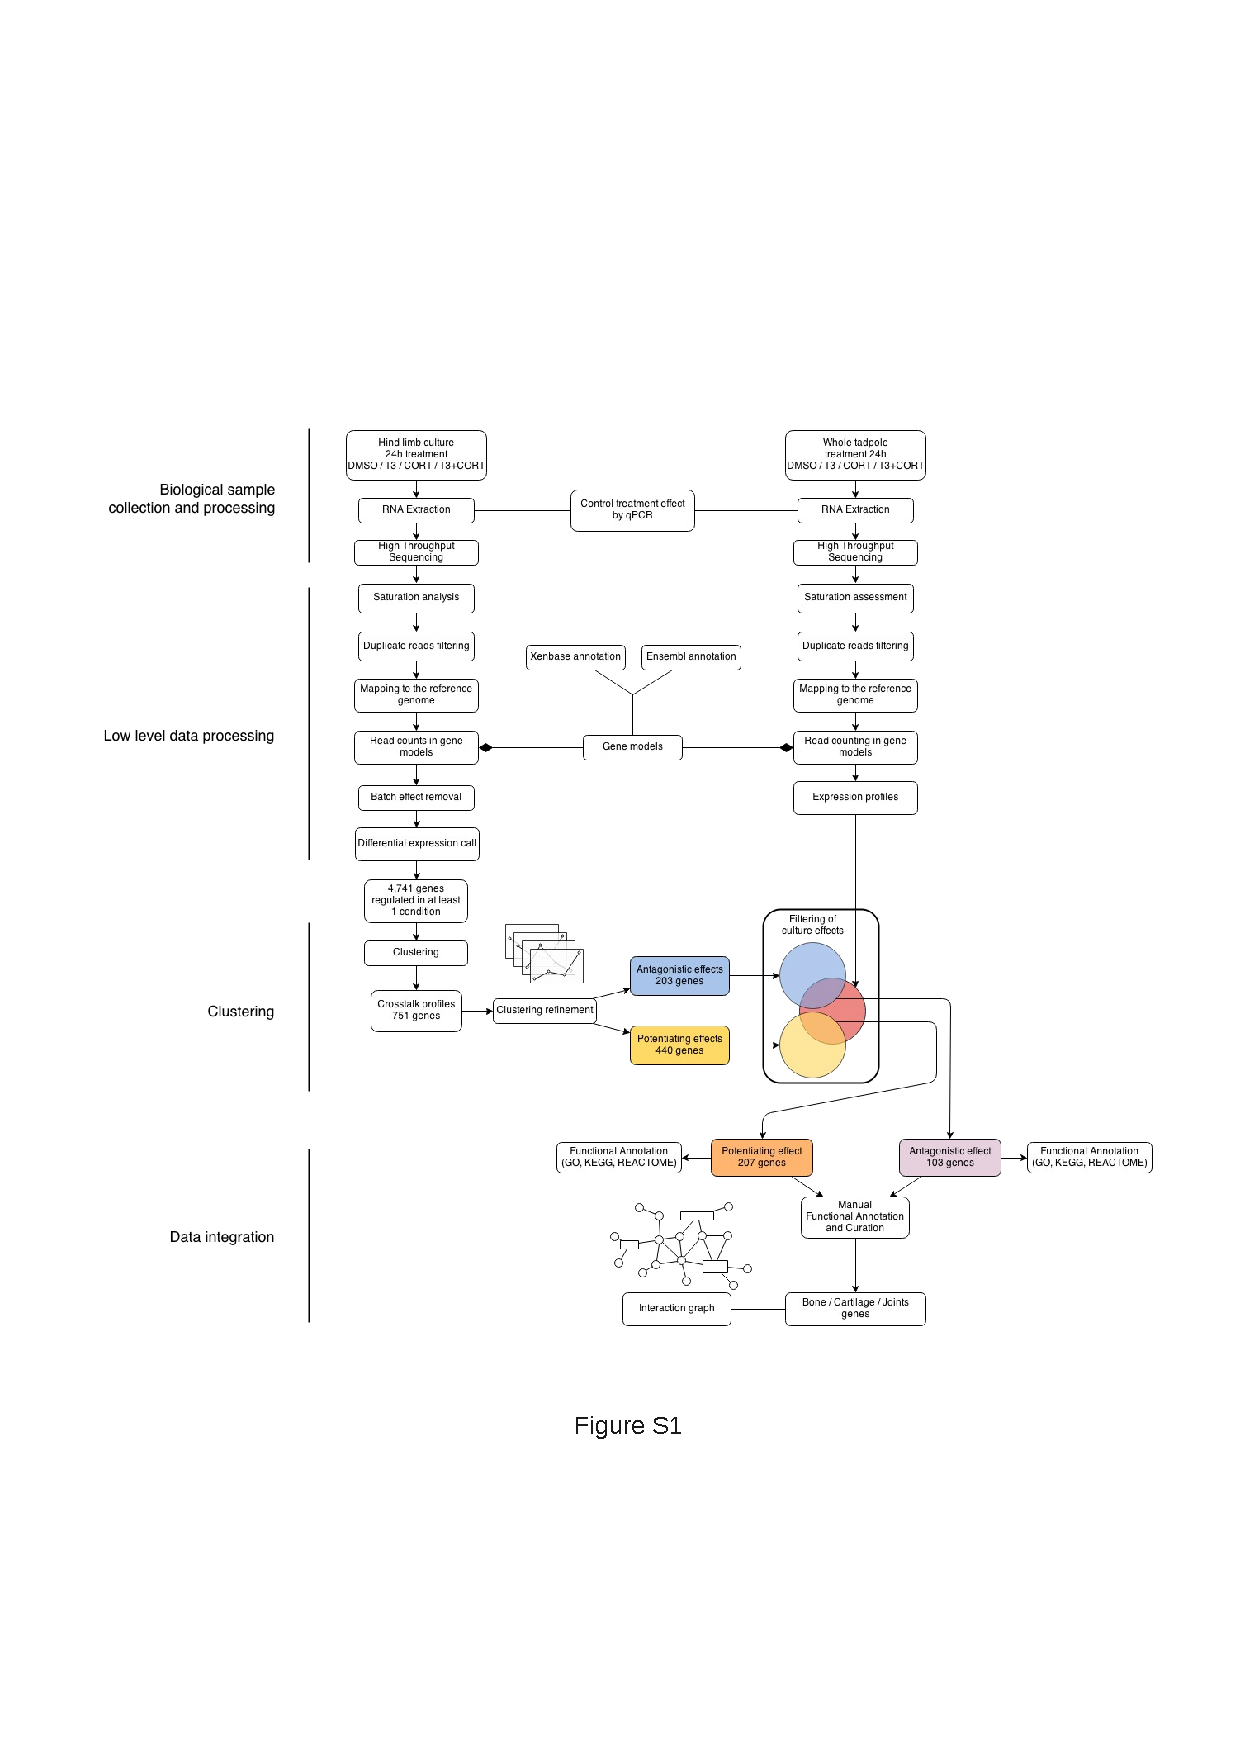
\includepdf[pages={-}]{Publications/grimaldi2014-sup.pdf}
	% }


% --- END - Article
% -----------------------------------------

% :::::::::::::::::::::::::::::::::::::::::

% -----------------------------------------
% --- 

\section{Annotation fonctionnelle automatique des termes enrichis dans les différentes catégories de profils d'expression}\label{sec:hlc-preanalysis}

% -----------------------------------------
% +++ BEGIN - Analyse globale

	\subsection{Analyse globale}
		La répartition des gènes dans les différents types de profils d'expression sont hétérogènes.
		Seule une minorité est affectée par le traitement aux \glspl{gc} (\autoref{fig:hlc-heatmap-de-genes} et Figure 1 de l'article en \autoref{subsec:grimaldi2014}).
		La majeure partie des profils d'expression des gènes différentiellement exprimés correspond ainsi à un effet du traitement à la \gls{t3}.
		Une minorité de gènes sont toutefois classifiés comme ayant une une réponse à la \gls{cort}, aussi bien seule que interagissant avec la réponse à la \gls{t3}.

		% BOTTOM caption
% ------------------------
%\begin{figure}[!htbp]
%\centering
%\vspace{1\baselineskip}
%\includegraphics[width=\textwidth]
% ------------------------
%
% SIDE caption
% ------------------------
\begin{SCfigure}[\sidecaptionrelwidth][!htbp]
\centering
%\vspace{1\baselineskip}
\includegraphics[width=0.5\textwidth]
% ------------------------
%
% Main information
% ===========================================================
{Figures/hlc-heatmap-de-genes/hlc-heatmap-de-genes.png}
\caption[Heatmap groupant 81 clusters de gènes ayant des profils d'expression similaires dans les bourgeons de pattes postérieures]
{
Heatmap groupant 81 clusters de gènes ayant des profils d'expression similaires dans les bourgeons de pattes postérieures.
Chaque ligne représente un cluster de gènes déterminé par "fuzzy c-mean clustering" (voir \autoref{sec:grimaldi2014}, "Materials \& Methods").
Le niveau d'expression de chaque cluster est centré sur zero, et la variance à travers les quatre traitements ajustée à un.
Le dendrogramme et l'ordre des clusters est calculé sur la base de leur distance euclidienne.
Les chiffres à gauche du dendrogramme correspondent aux numéros des clusters.
}
\label{fig:hlc-heatmap-de-genes}
% ===========================================================
%
% BOTTOM caption
% ------------------------
%\end{figure}
% ------------------------
%
% SIDE caption
% ------------------------
\end{SCfigure}
% ------------------------
%
%\missingfigure{Make a figure}

		L'annotation fonctionnelle automatisée des gènes différentiellement exprimés dans au moins une condition (4741 gènes) a été réalisée avec l'outil en ligne GOrilla en utilisant l'ensemble des gènes exprimés comme ``background''.
		Il en ressort un fort enrichissement en termes associés au métabolisme des lipides, du cycle cellulaire, du système immunitaire, des \glspl{rna} et au transport intra-cellulaire de molécules (\autoref{fig:hlc-go-all-graph}).
		Cette représentation est particulièrement adaptée à l'illustration des résultats obtenus.
		En effet, elle permet d'intégrer les relations entre les différents termes présentés.
		Ceci permet de facilement évaluer le rôle plus ou moins fin des gènes considérés (à condition que l'annotation soit complète) dans le contexte de fonctions biologiques ou moléculaires plus générales.

		\begin{sidewaysfigure}[p]
\begin{subfigure}{\textwidth}
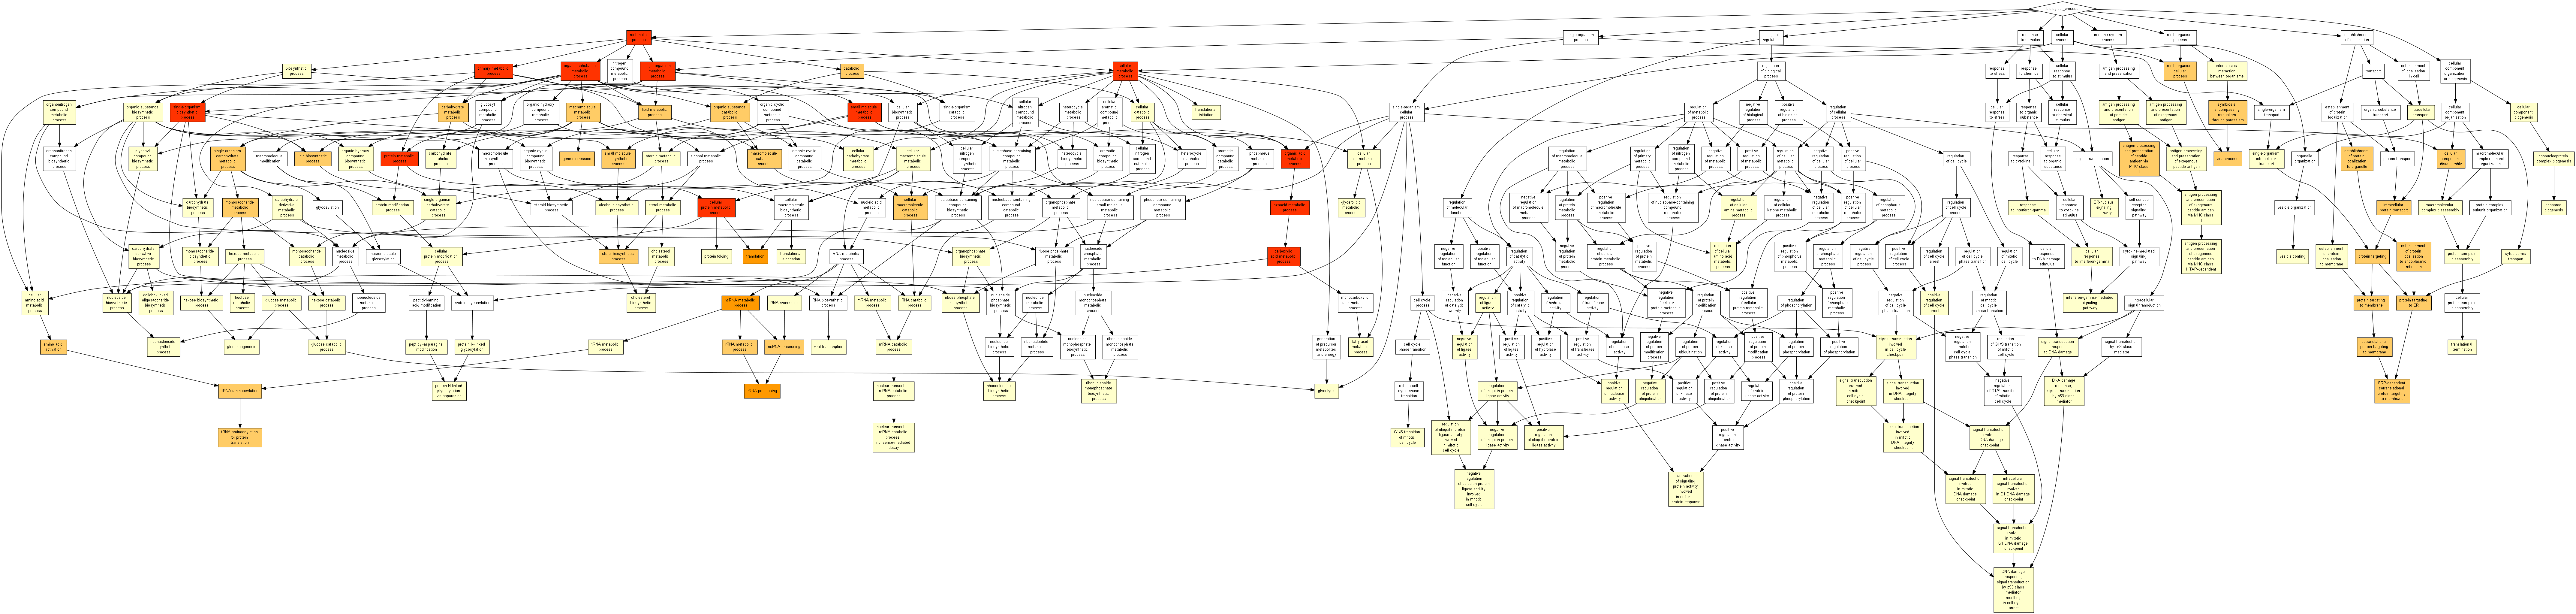
\includegraphics[width=\textwidth]
{Figures/hlc-go-all-graph/hlc-go-all-graph.png}
\caption{Vue générale}
\end{subfigure}
\end{sidewaysfigure}

\begin{figure}[p]
\ContinuedFloat
\begin{subfigure}{\textwidth}
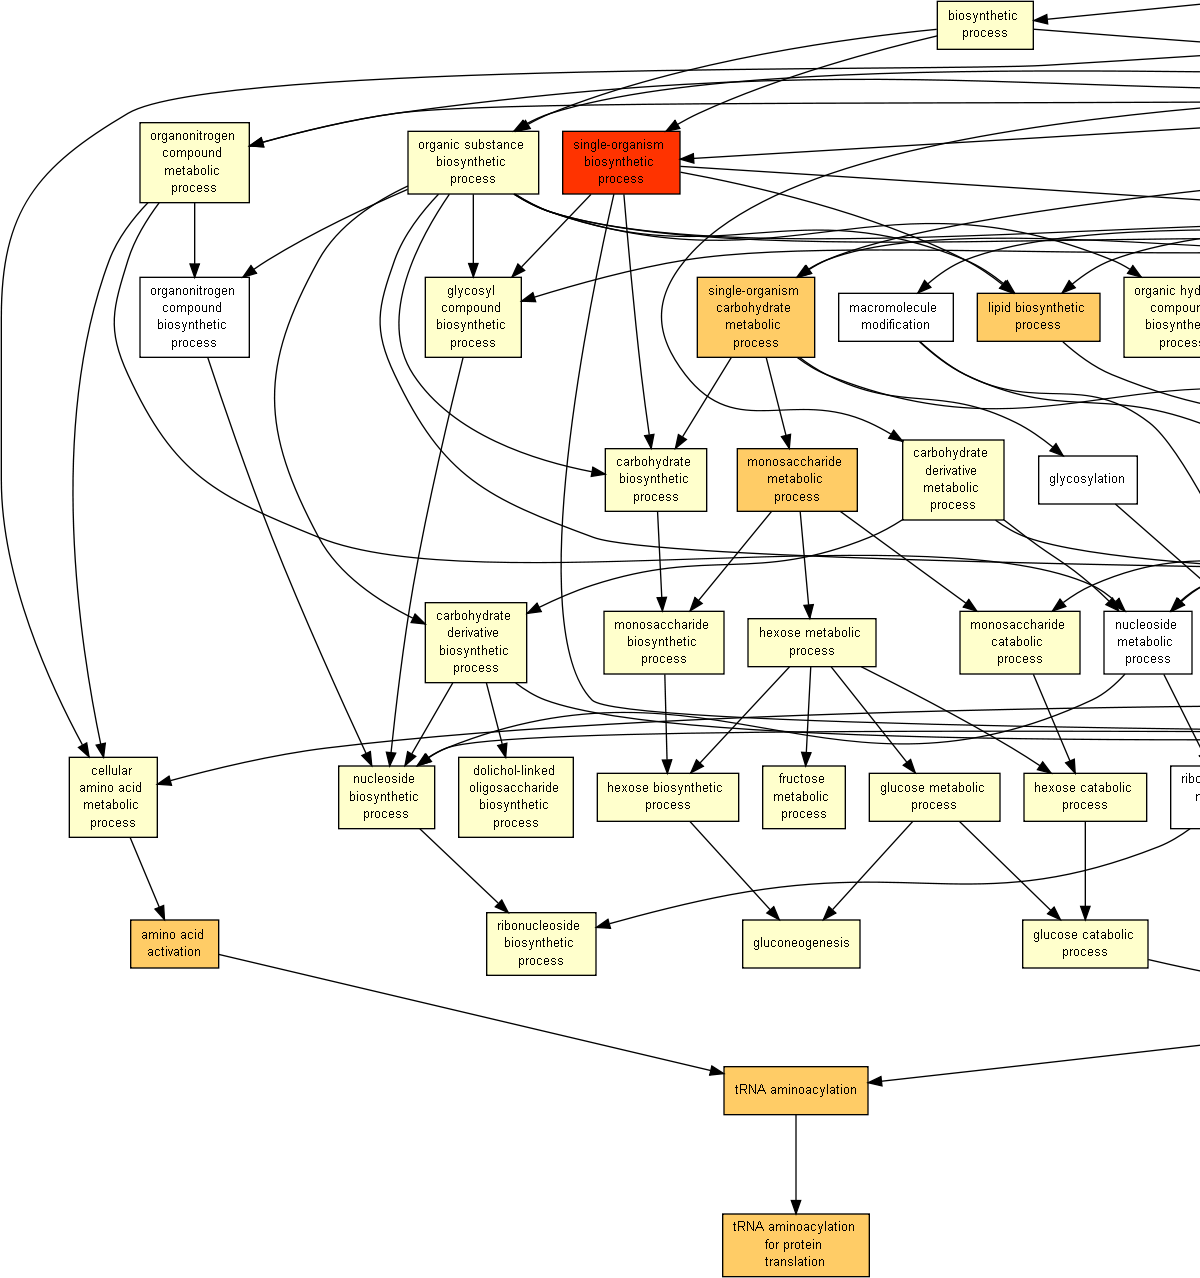
\includegraphics[width=\textwidth]
{Figures/hlc-go-all-graph/hlc-go-all-graph_0.png}
\caption{1/8}
\end{subfigure}
\end{figure}

\begin{figure}[p]
\ContinuedFloat
\begin{subfigure}{\textwidth}
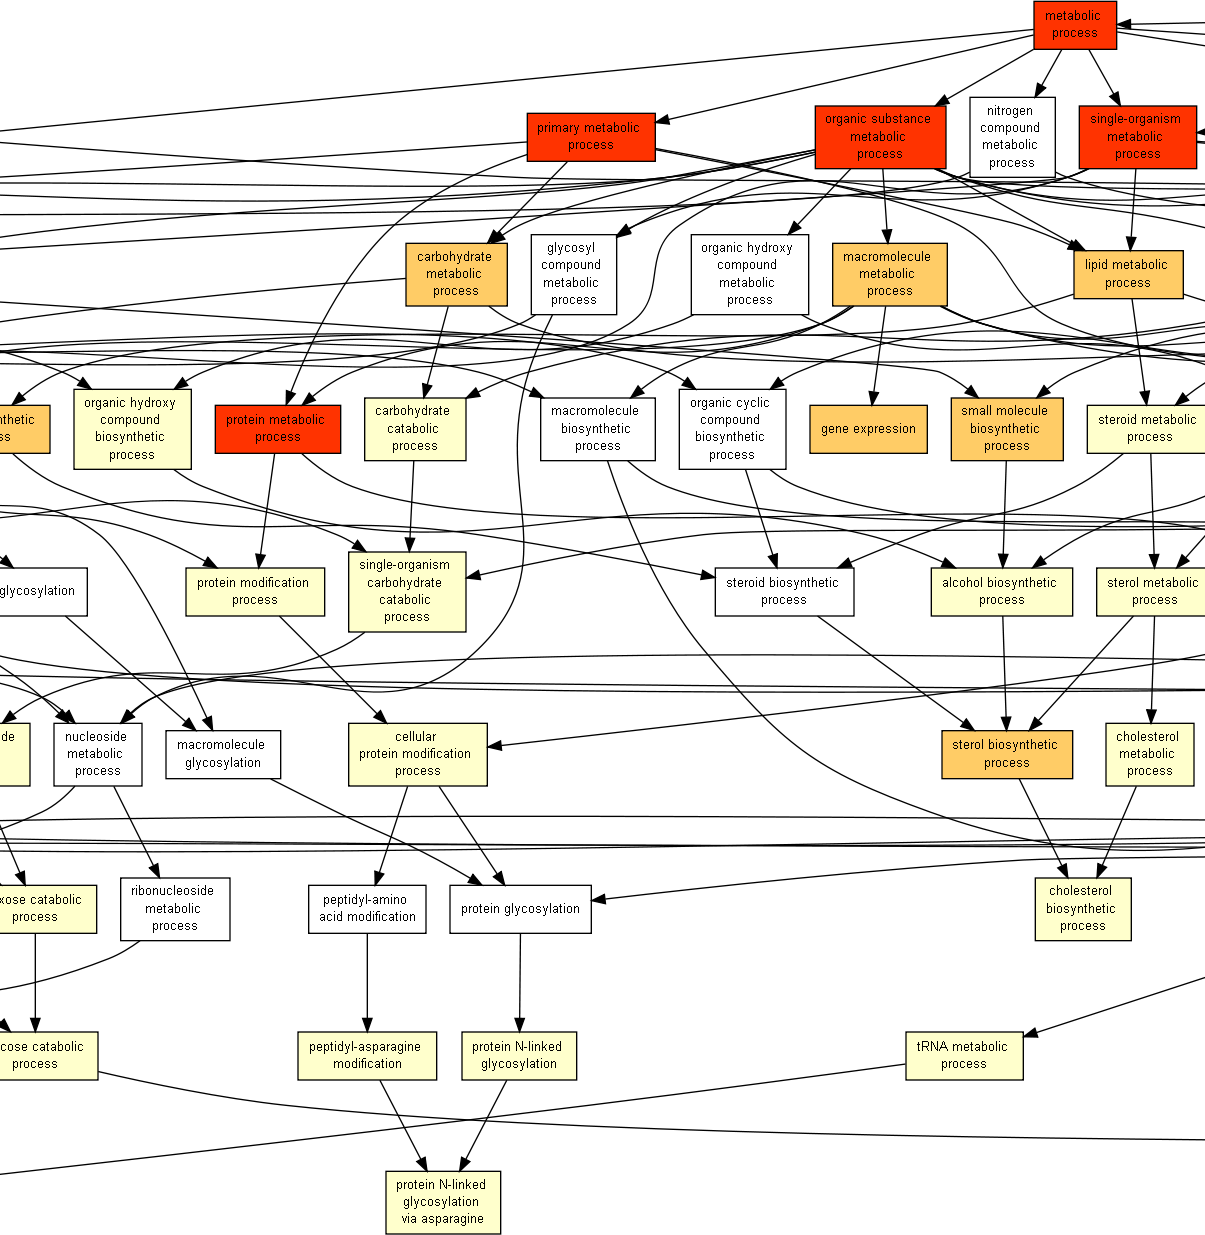
\includegraphics[width=\textwidth]
{Figures/hlc-go-all-graph/hlc-go-all-graph_1.png}
\caption{2/8}
\end{subfigure}
\end{figure}

\begin{figure}[p]
\ContinuedFloat
\begin{subfigure}{\textwidth}
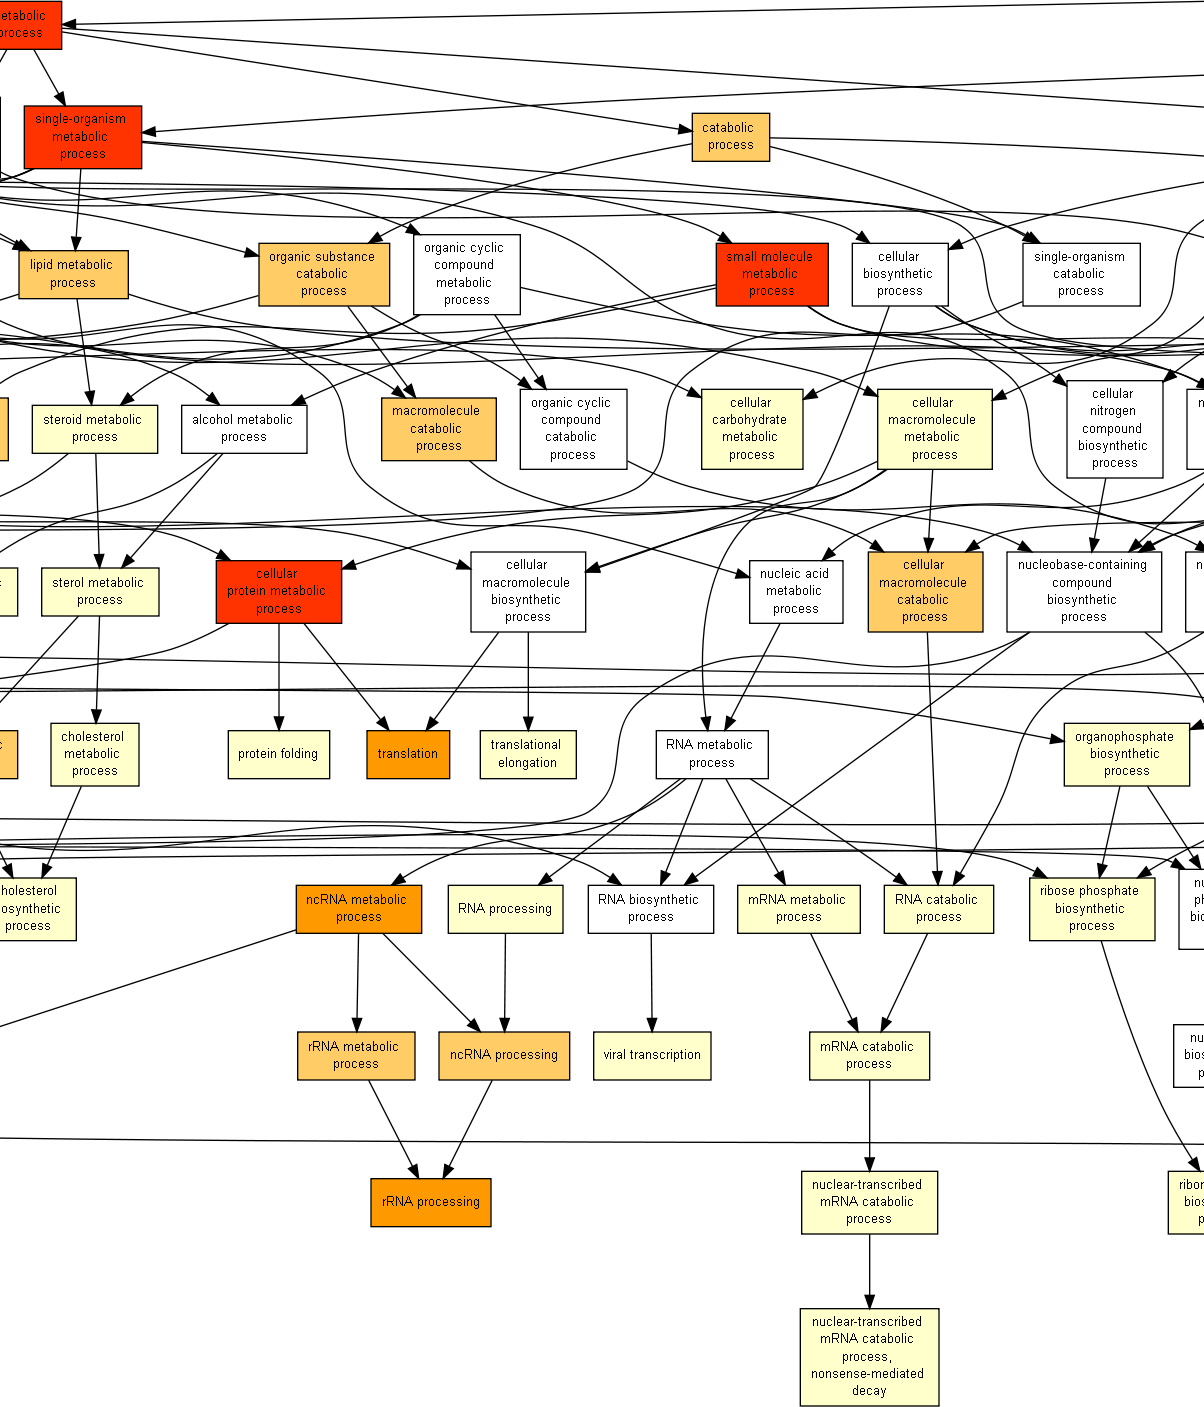
\includegraphics[width=\textwidth]
{Figures/hlc-go-all-graph/hlc-go-all-graph_2.png}
\caption{3/8}
\end{subfigure}
\end{figure}

\begin{figure}[p]
\ContinuedFloat
\begin{subfigure}{\textwidth}
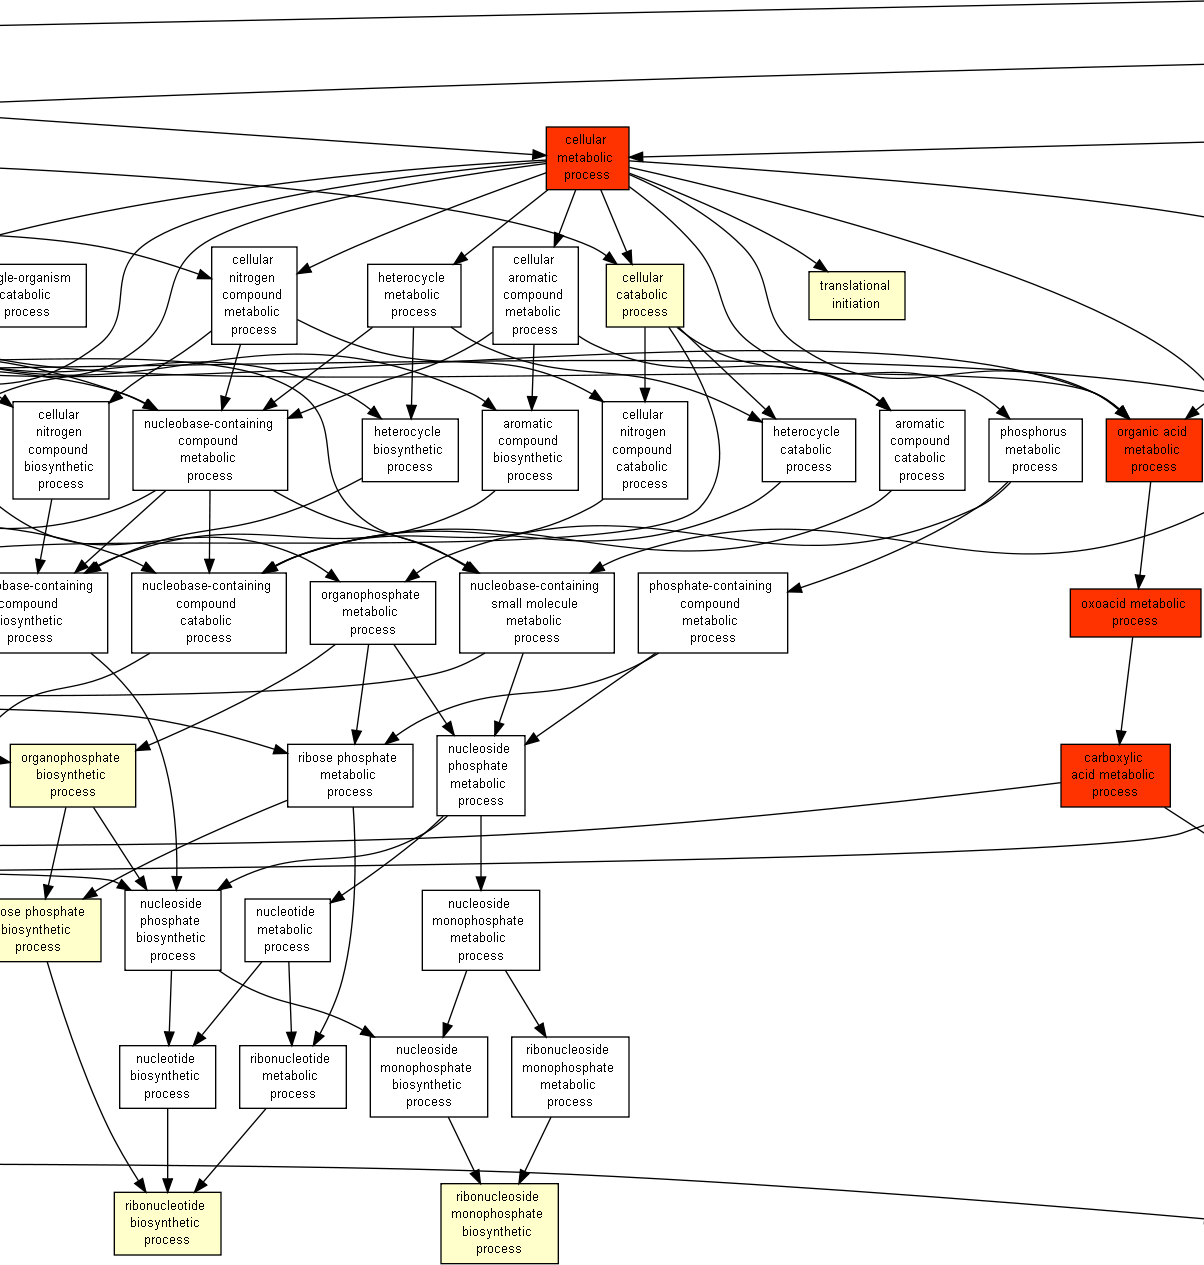
\includegraphics[width=\textwidth]
{Figures/hlc-go-all-graph/hlc-go-all-graph_3.png}
\caption{4/8}
\end{subfigure}
\end{figure}

\begin{figure}[p]
\ContinuedFloat
\begin{subfigure}{\textwidth}
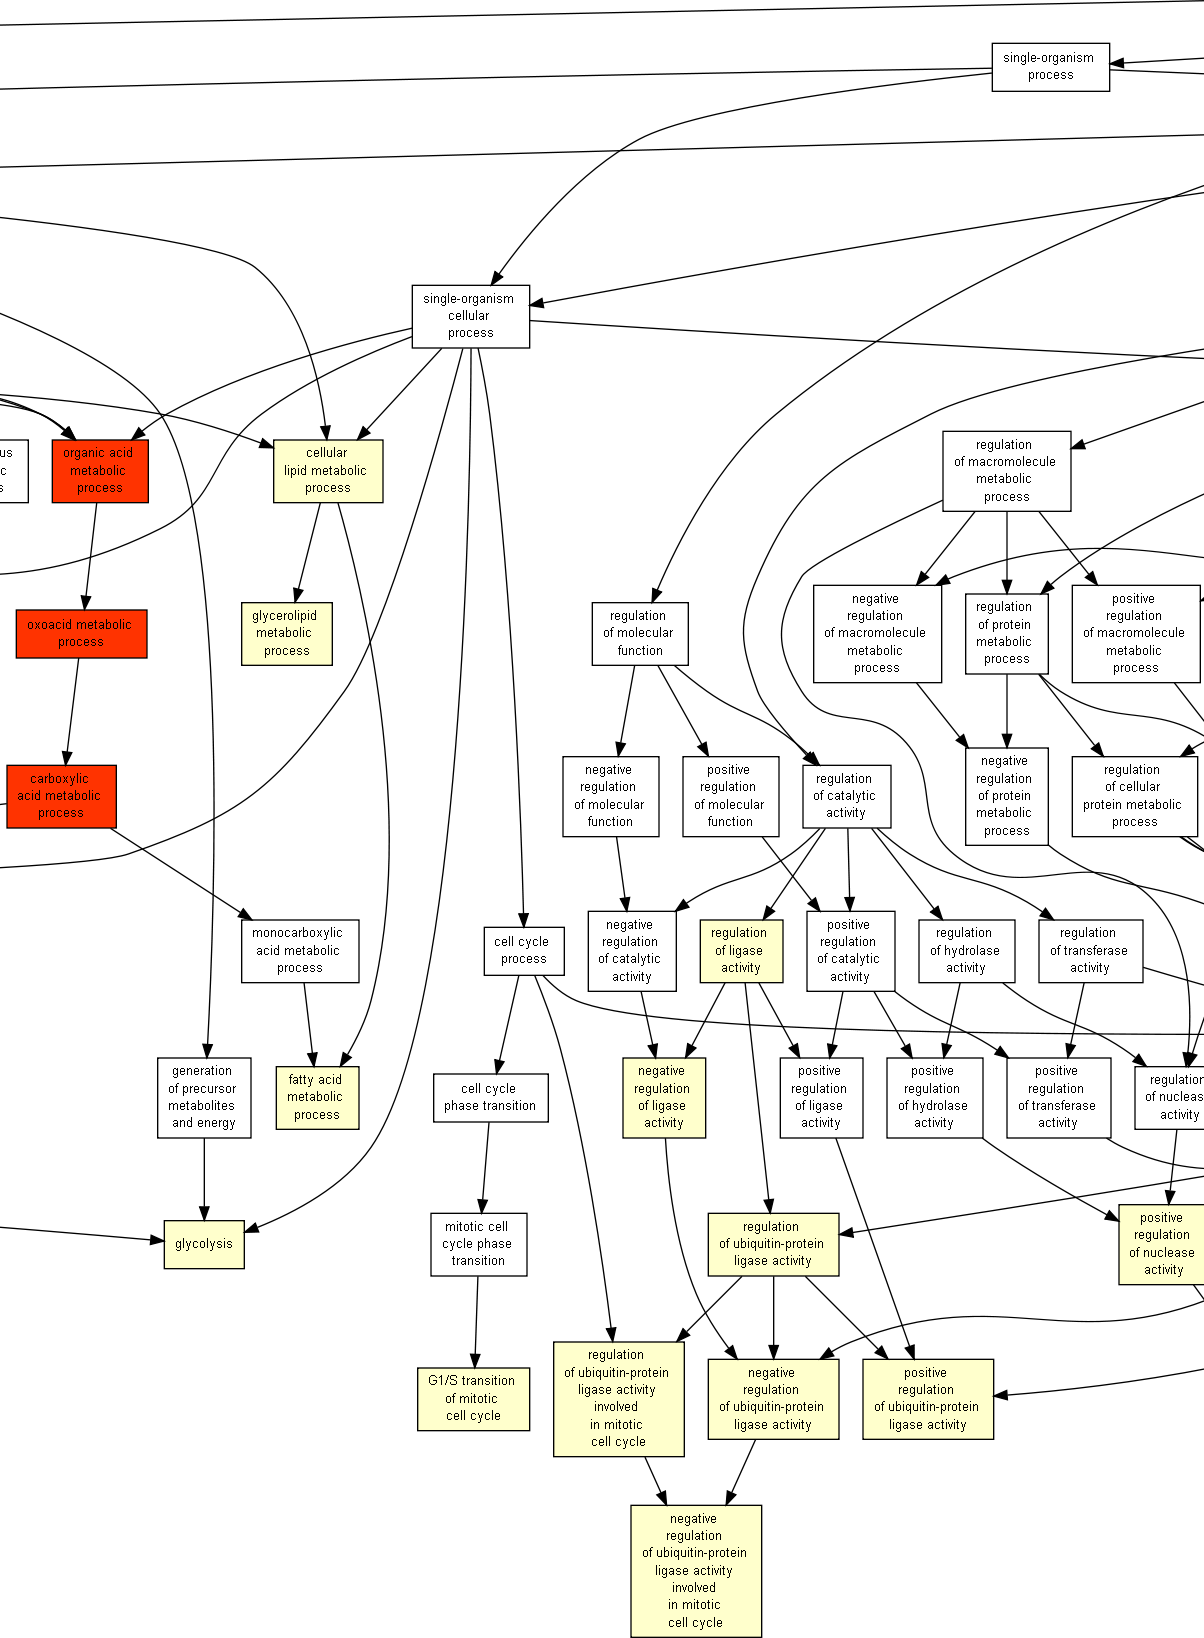
\includegraphics[width=\textwidth]
{Figures/hlc-go-all-graph/hlc-go-all-graph_4.png}
\caption{5/8}
\end{subfigure}
\end{figure}

\begin{figure}[p]
\ContinuedFloat
\begin{subfigure}{\textwidth}
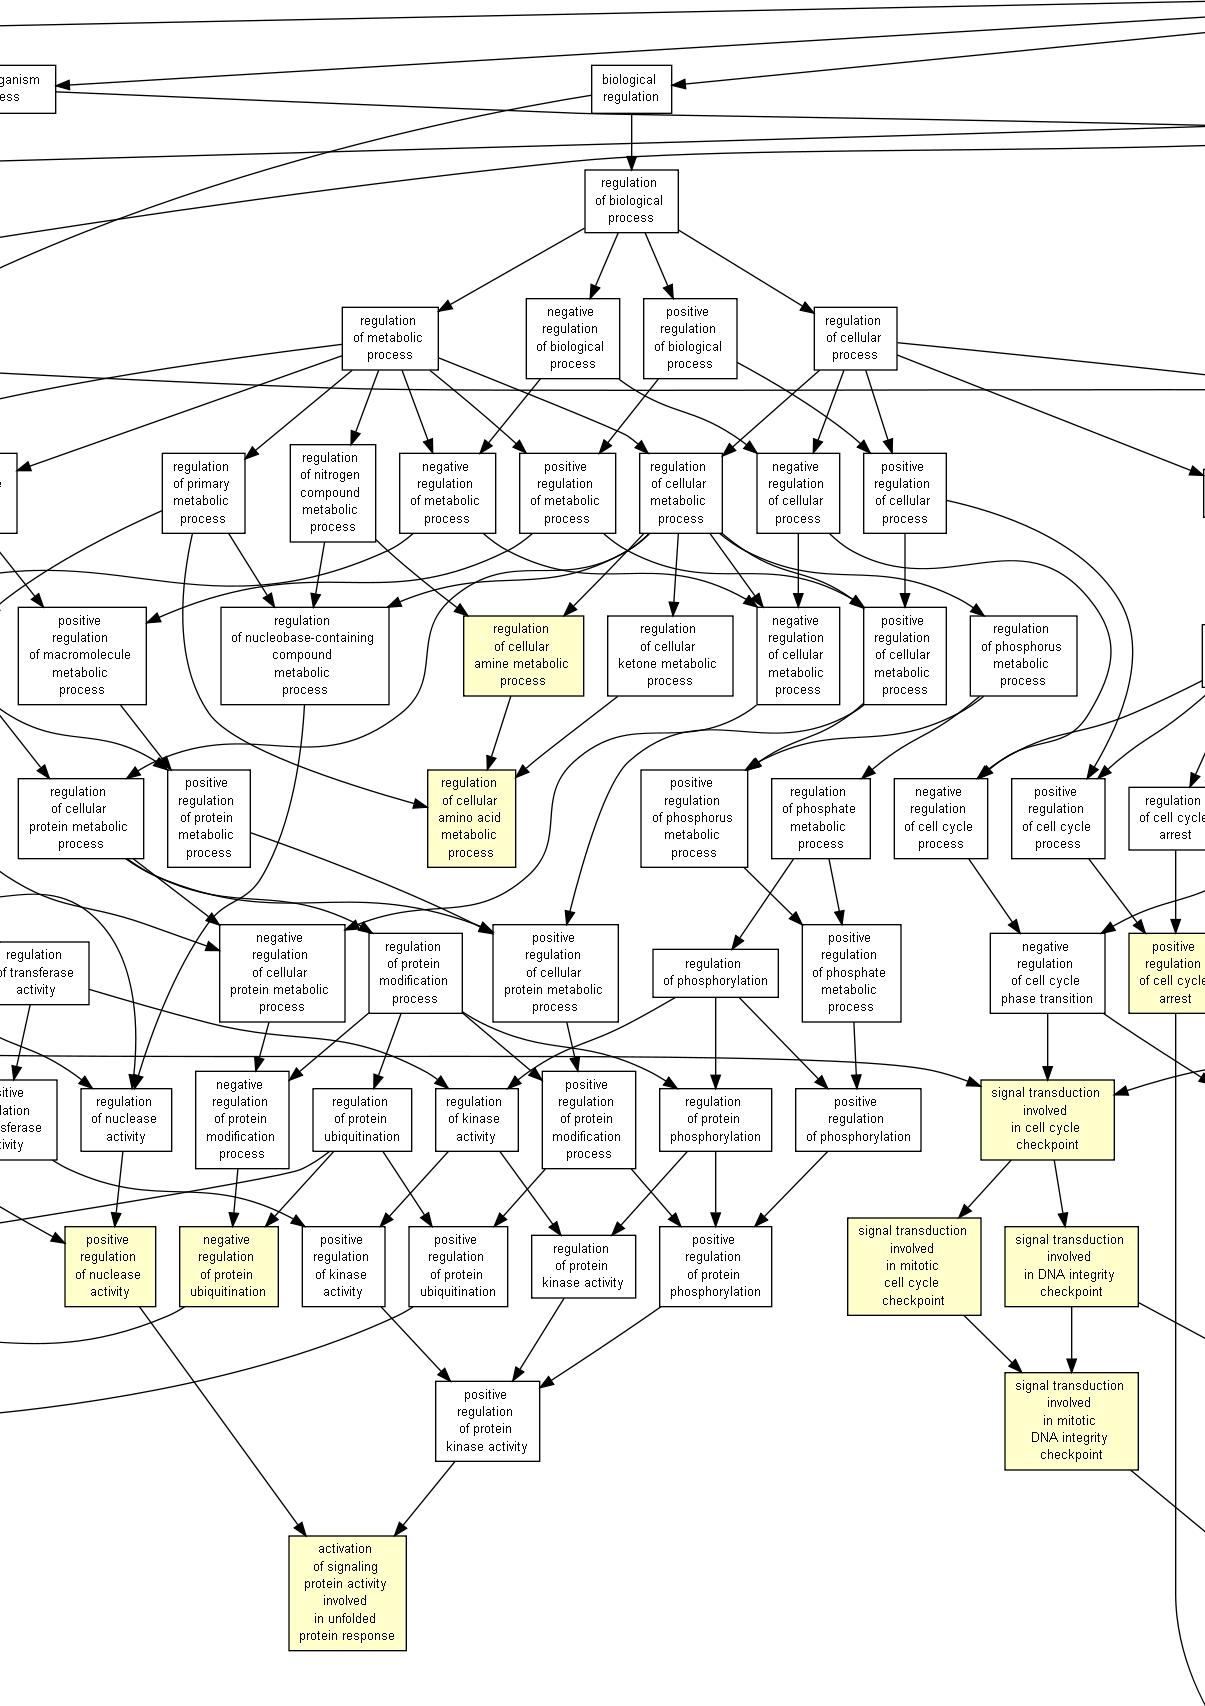
\includegraphics[width=\textwidth]
{Figures/hlc-go-all-graph/hlc-go-all-graph_5.png}
\caption{6/8}
\end{subfigure}
\end{figure}

\begin{figure}[p]
\ContinuedFloat
\begin{subfigure}{\textwidth}
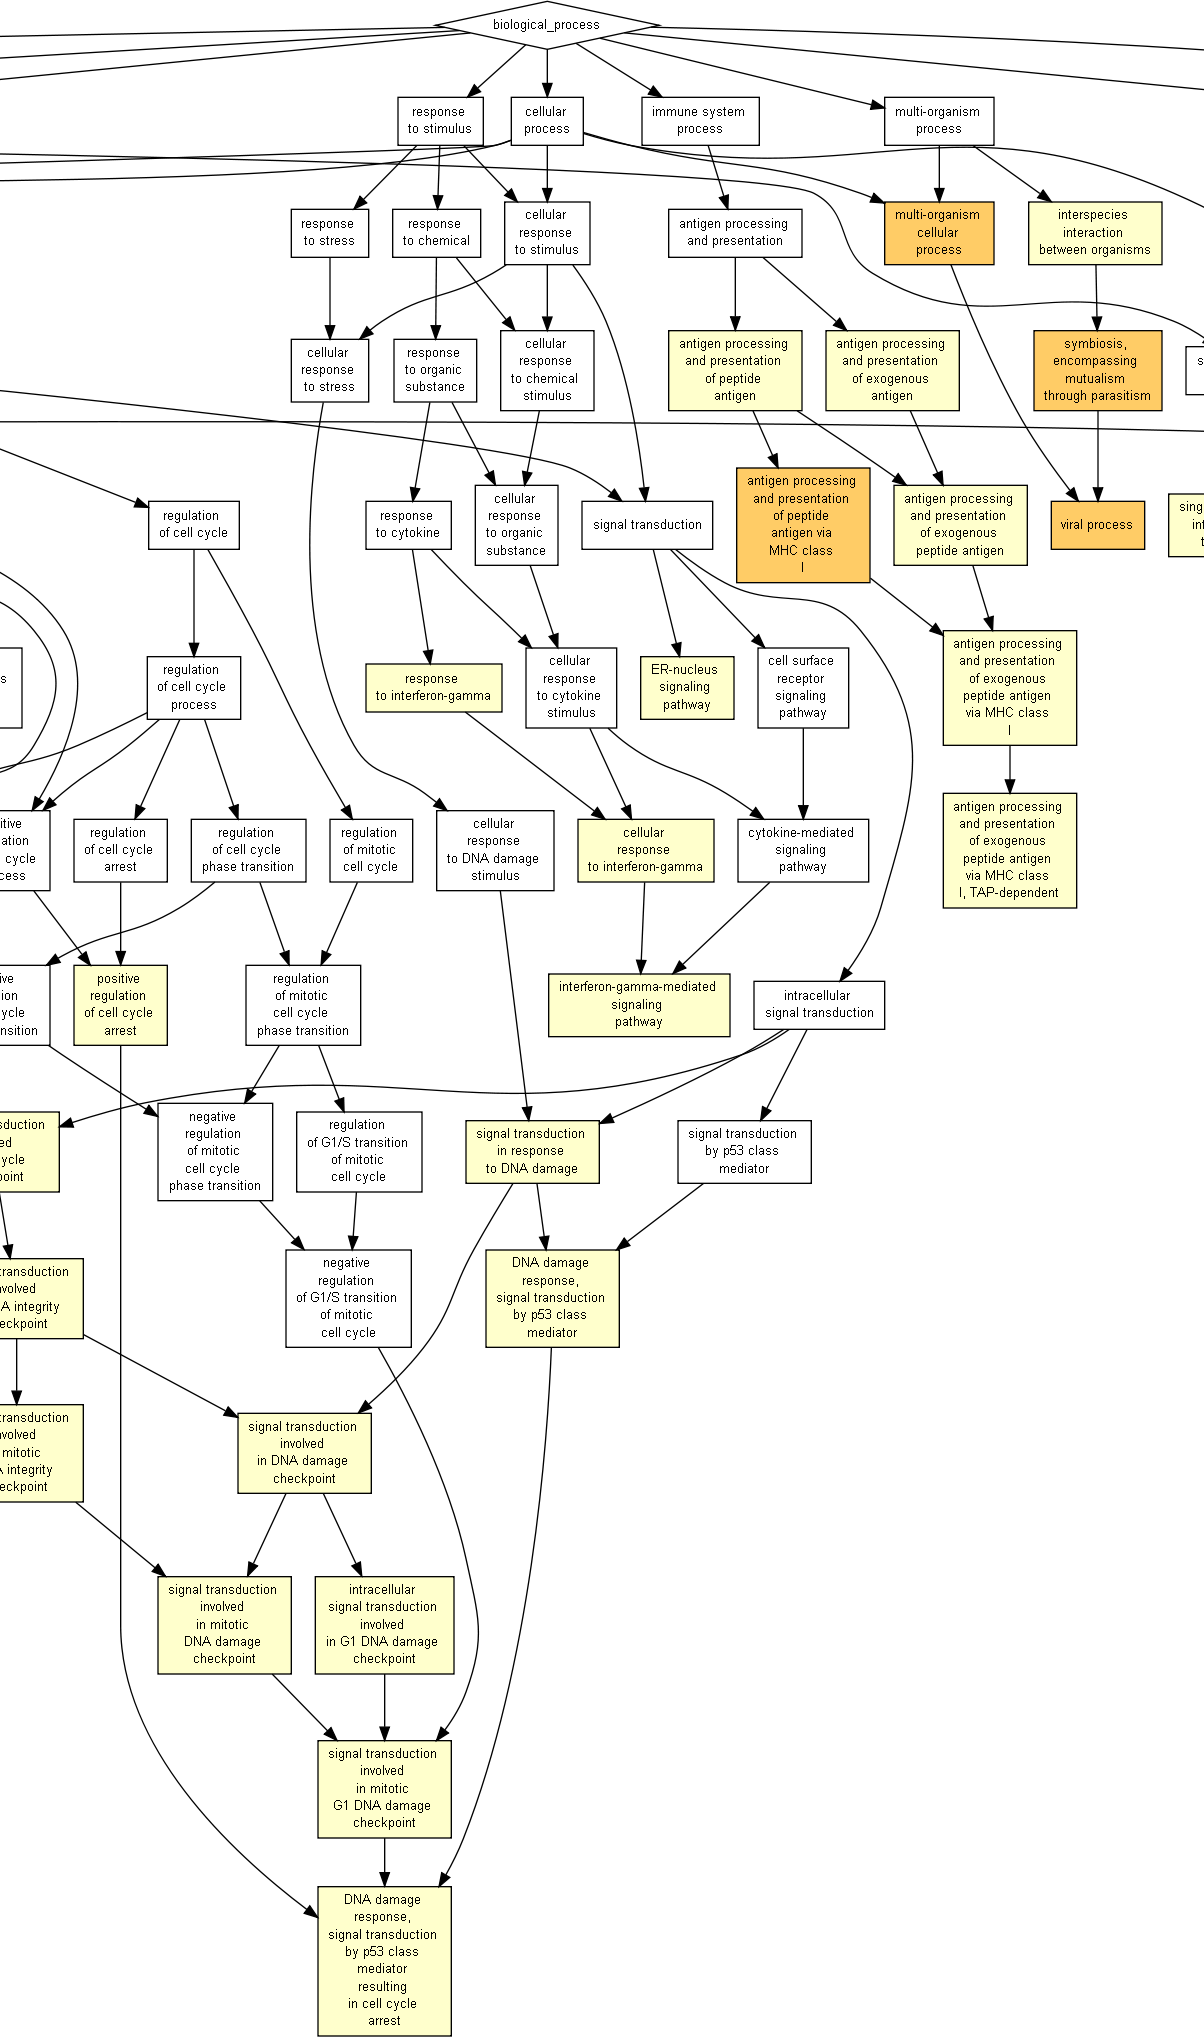
\includegraphics[width=\textwidth]
{Figures/hlc-go-all-graph/hlc-go-all-graph_6.png}
\caption{7/8}
\end{subfigure}
\end{figure}

\begin{figure}[!htp]
%\begin{sidewaysfigure}[!htbp]
\ContinuedFloat
\begin{subfigure}{\textwidth}
\includegraphics[width=\textwidth]
%{Figures/hlc-go-all-graph/hlc-go-all-graph.png}
{Figures/hlc-go-all-graph/hlc-go-all-graph_7.png}
\caption{8/8}
\end{subfigure}
\caption[Enrichissement des catégories fonctionnelles associées aux gènes différentiellement exprimés dans les bourgeons de pattes postérieures]
{
(Neuf pages précédentes) Enrichissement des catégories fonctionnelles associées aux gènes différentiellement exprimés dans les bourgeons de pattes postérieures.
a) Vue générale.
b) Détail.
L'enrichissement des termes comparé à l'ensemble des gènes transcrits est calculé à l'aide de GOrilla \citep{Eden2009}.
Les couleurs des boites correspondent à la significativité de l'enrichissement.
Jaune pâle : $10^{-3} \leq p < 10^{-5}$
Jaune : $10^{-5} \leq p < 10^{-7}$
Orange : $10^{-7} \leq p < 10^{-9}$
Rouge: $p < 10^{-9}$
}
\label{fig:hlc-go-all-graph}
%\end{sidewaysfigure}
\end{figure}

		Une représentation condensée mets l'accent sur les catégories sur-représentées dans une hiérarchie simplifiée à 2 niveaux (\autoref{fig:hlc-go-all-treemap}):
		Plusieurs processus biologiques sont affectés par le traitement hormonal.
		Tout d'abord, le métabolisme des lipides et les voies de biosynthèse des dérivés carbohydrates et stéroïdes.
		La régulation fine des \glspl{rna} et leur traduction semble aussi affectée, avec un effet sur des facteurs régulant le temps de demi-vie des \gls{rna} et des facteurs impliquées dans le métabolisme des \gls{rrna} et des \gls{ncrna}.
		Enfin, la physiologie de la cellule est affectée notamment au niveau du cytosquelette et du trafic intra-cellulaire.
		Dans une moindre mesure, le système immunitaire est également affecté, ainsi que des aspects généraux du métabolisme.

		\begin{sidewaysfigure}[!htbp]
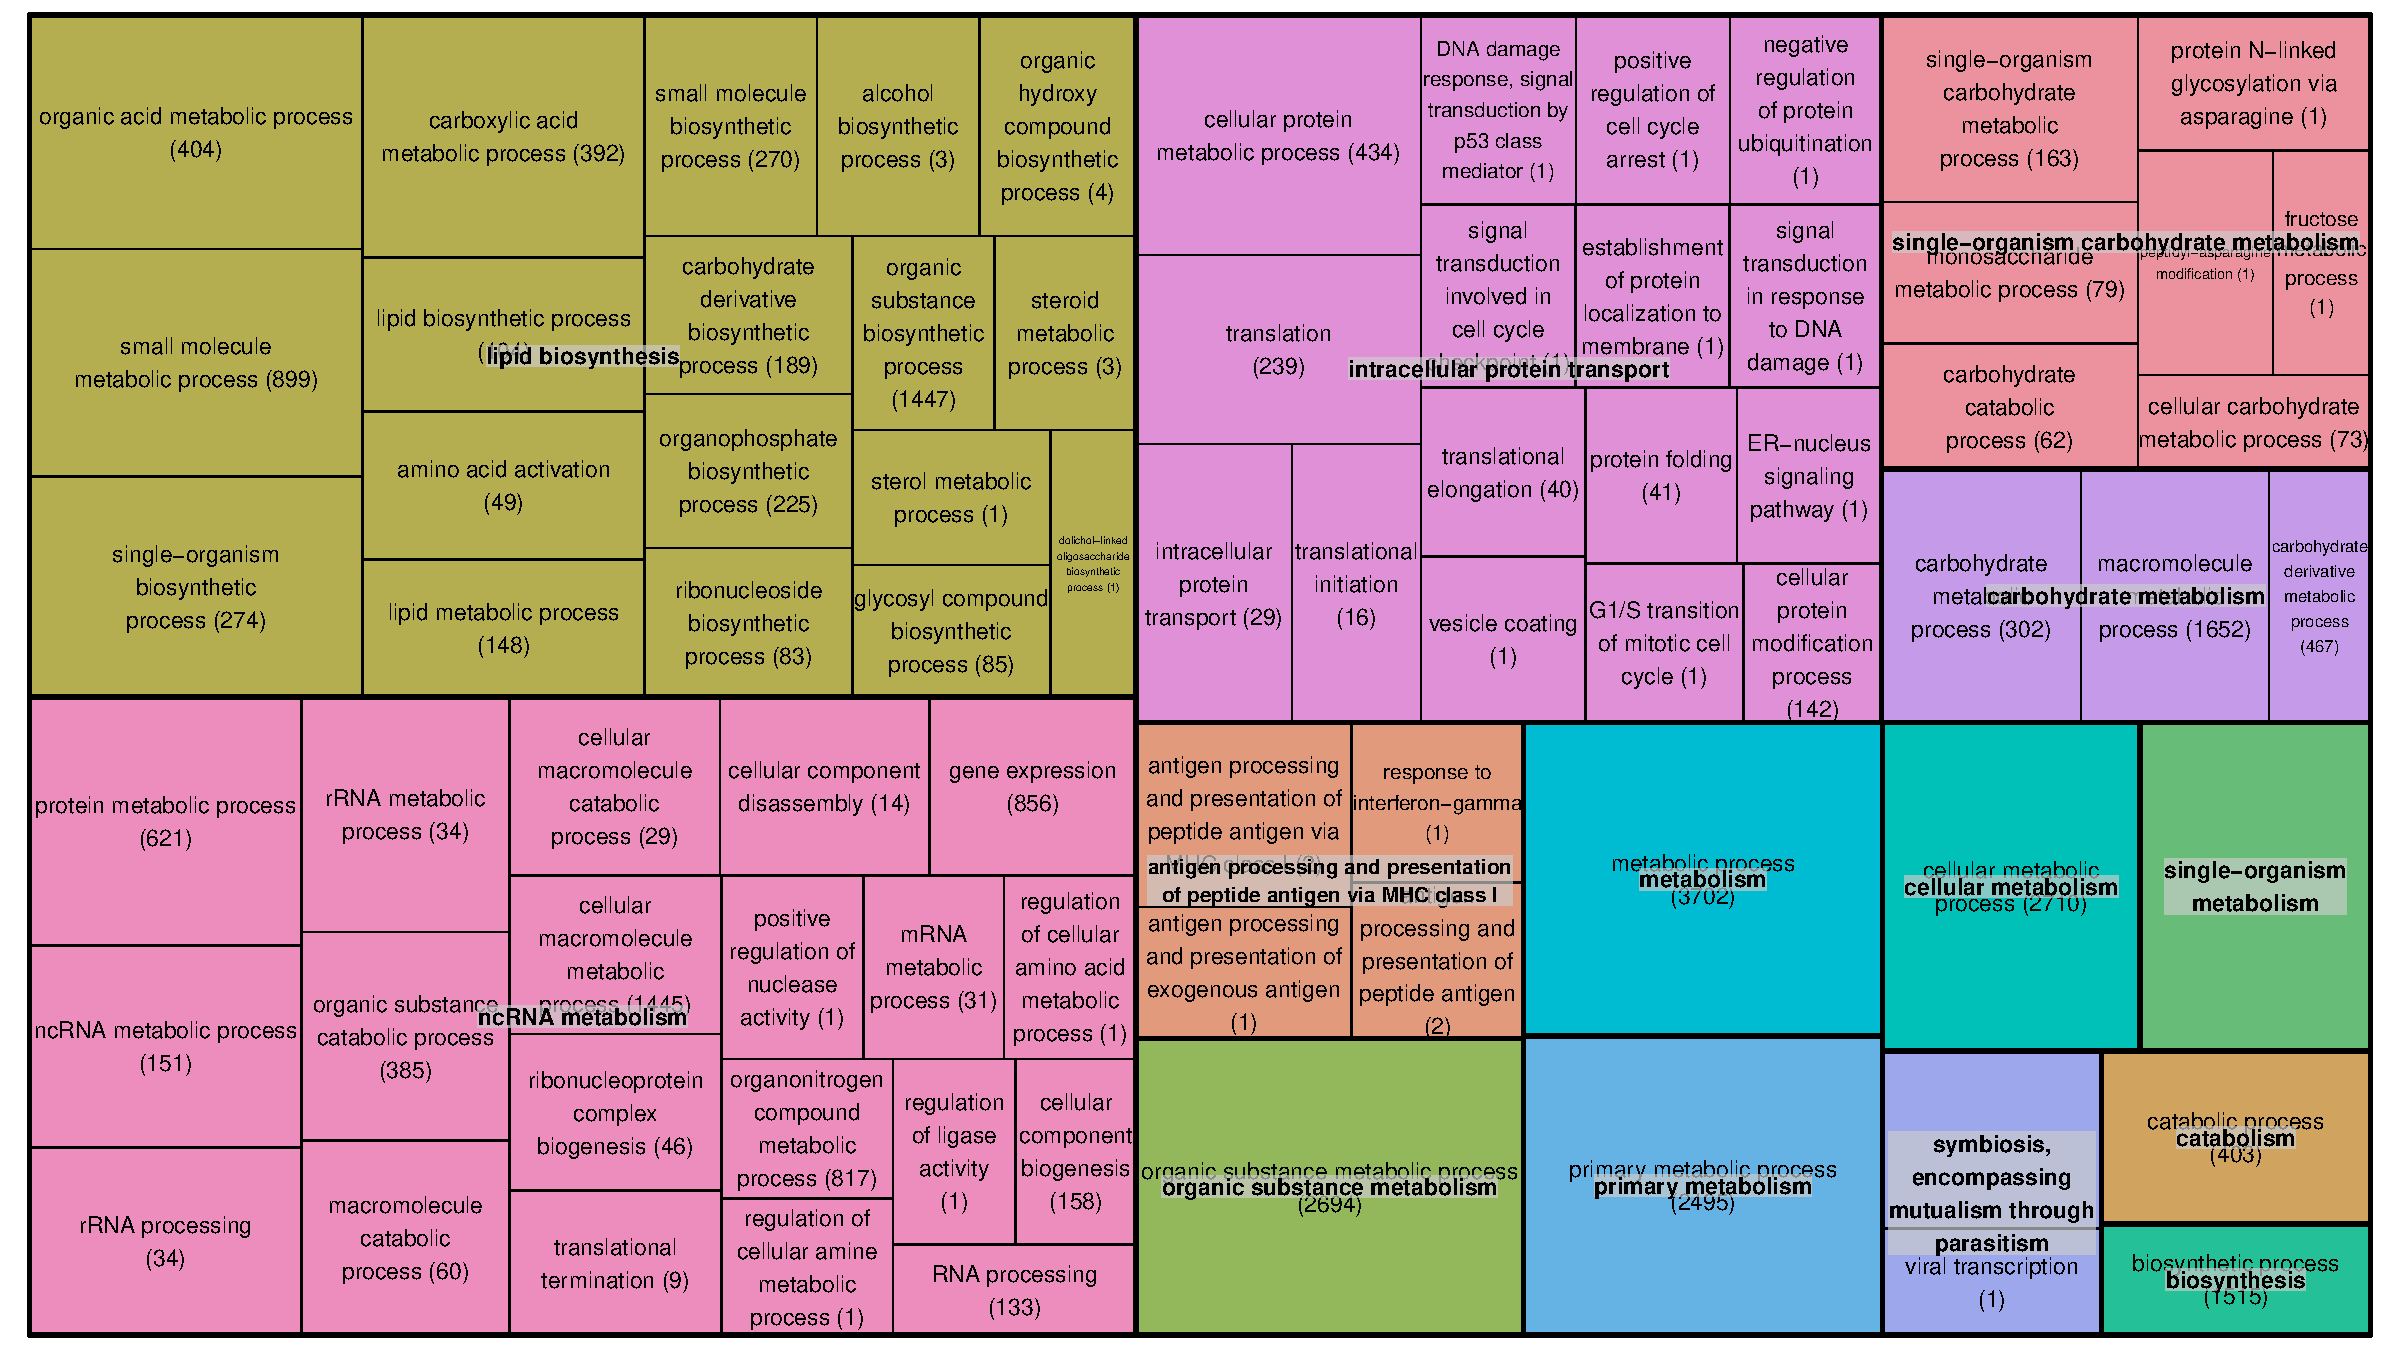
\includegraphics[width=\textwidth]
{Figures/hlc-go-all-treemap/hlc-go-all-treemap.pdf}
\caption[Enrichissement des catégories fonctionnelles associées aux gènes différentiellement exprimés dans les bourgeons de pattes postérieures]
{
Enrichissement des catégories fonctionnelles associées aux gènes différentiellement exprimés dans les bourgeons de pattes postérieures.
L'enrichissement de catégories fonctionnelles obtenu \autoref{fig:hlc-go-all-graph} a subit un post-traitement à l'aide de REViGO \citep{Supek2011} afin de résumer les différentes catégories avec une granularité moindre (deux niveaux) et de les représenter sous forme de "treemap".
La taille des rectangles est proportionnelle à la significativité de l'enrichissement de la catégorie fonctionnelle associée.
Le nombre de gènes associé à chaque catégorie est indiqué dans chaque cadre.
Un gène pouvant être associé à plusieurs catégories, le total du nombre de gènes indiqué dans chaque case est supérieur au nombre de gènes utilisé en entrée.
}
\label{fig:hlc-go-all-treemap}
\end{sidewaysfigure}

	% -----------------------------------------
	% +++ BEGIN - Interactions entre hormones

	\subsection{Analyse des clusters spécifiques d'une interaction croisée entre les effets des deux hormones}
		Après avoir fait le choix délibéré de concentrer l'analyse sur les gènes affectés par les deux hormones simultanément (Figure 2 de l'article à la \autoref{subsec:grimaldi2014}, Figure 2), j'ai répété l'annotation fonctionnelle des gènes dans les différentes catégories de profil d'expression, parmi les profils "antagonistes" et ``potentiation'' en distinguant dans chaque cas les gènes induits et les gènes réprimés.
		Le contraste utilisé à cette étape emploie l'ensemble des 4741 gènes différentiellement exprimés dans au moins une condition comme background.
		Ceci permet de capturer les termes enrichis dans le contexte d'une intéraction croisée particulière comparée à ceux enrichis dans le contexte d'un effet quelconque.
		De façon frappante, le contenu en gènes dans ces quatre catégories sous-tend des processus biologiques contrastés.

	% -----------------------------------------
	% +++ BEGIN - Clusters antagoniste

		\subsubsection{Gènes ``antagonisés''}

			\paragraph{Gènes dont la répression \gls{t3}-dépendante est antagonisée par la \gls{cort}}
				Dans cette catégorie, le contenu en gène ne semble pas enrichi de façon dramatique en une fonction biologique particulière, malgré la participation de \gls{aadac} et \gls{pnpla2} au métabolisme des tri-glycérides (\autoref{fig:hlc-go-antago-down}, $\textit{p} = 2,05 * 10^{-4}$ pour les deux termes).

				% BOTTOM caption
% ------------------------
\begin{figure}[!htbp]
\centering
\vspace{1\baselineskip}
\includegraphics[width=\textwidth]
% ------------------------
%
% SIDE caption
% ------------------------
%\begin{SCfigure}[\sidecaptionrelwidth][!htbp]
%\centering
%\vspace{1\baselineskip}
%\includegraphics[width=0.5\textwidth]
% ------------------------
%
% Main information
% ===========================================================
{Figures/hlc-go-antago-down/hlc-go-antago-down.png}
\caption[Enrichissement fonctionnel des gènes dont la répression des gènes \gls{ht}-dépendante est inhibée par les \glspl{gc}]
{
Termes enrichis parmis les fonctions biologues associées aux gènes réprimés par la \gls{t3} dans les clusters "antagonistes".
Les couleurs des boites correspondent à la significativité de l'enrichissement.
Jaune pâle : $10^{-3} \leq 10^{-5}$
Jaune : $10^{-5} \leq p < 10^{-7}$
Orange : $10^{-7} \leq p < 10^{-9}$
Rouge: $p < 10^{-9}$
}
\label{fig:hlc-go-antago-down}
% ===========================================================
%
% BOTTOM caption
% ------------------------
\end{figure}
% ------------------------
%
% SIDE caption
% ------------------------
%\end{SCfigure}
% ------------------------

			\paragraph{Gènes dont l'induction \gls{t3}-dépendante est antagonisée par les \gls{cort}}
				Cette catégorie non-plus ne présente pas d'enrichissement fonctionnel fort.
				\gls{mcm4}, \gls{mcm2} et \gls{lig1} participent cependant à la légère sur-représentation du contrôle de la réplication de l'\gls{dna} (\autoref{fig:hlc-go-antago-up}, $\textit{p}=3,36*10^{-5}; \textit{p}=4,35*10^{-5}\textit{p}=4,53*10^{-4}$ pour les trois termes).

				% BOTTOM caption
% ------------------------
\begin{figure}[!htbp]
\centering
\vspace{1\baselineskip}
\includegraphics[width=\textwidth]
% ------------------------
%
% SIDE caption
% ------------------------
%\begin{SCfigure}[\sidecaptionrelwidth][!htbp]
%\centering
%\vspace{1\baselineskip}
%\includegraphics[width=0.5\textwidth]
% ------------------------
%
% Main information
% ===========================================================
{Figures/hlc-go-antago-up/hlc-go-antago-up.png}
\phantomcaption
\end{figure}
\begin{figure}[t]
\ContinuedFloat
\caption[Enrichissement fonctionnel des gènes dont l'induction des gènes \gls{ht}-dépendante est inhibée par les \glspl{gc}.]
{
(Page précédente) Termes enrichis parmi les fonctions biologiques associées aux gènes induits par la \gls{t3} dans les clusters ``antagonistes''.
Les couleurs des boites correspondent à la significativité de l'enrichissement.
Jaune pâle : $10^{-5} \leq p < 10^{-3}$
Jaune : $10^{-7} \leq p < 10^{-5}$
Orange : $10^{-9} \leq p < 10^{-7}$
Rouge: $p < 10^{-9}$
}
\label{fig:hlc-go-antago-up}
% ===========================================================
%
% BOTTOM caption
% ------------------------
\end{figure}
% ------------------------
%
% SIDE caption
% ------------------------
%\end{SCfigure}
% ------------------------

		% -----------------------------------------
		% +++ BEGIN - Cluster potentiés

		\subsubsection{Gènes ``potentiés''}

			\paragraph{Gènes dont l'effet inducteur de la \gls{t3} est potentié par la \gls{cort}}
				La seule catégorie fonctionnelle enrichie dans ce sous-ensemble de gènes correspond au développement de l'épiderme (\autoref{fig:hlc-go-pot-up}; gènes \gls{bnc1}, \gls{znf750}, \gls{krt17}, \gls{lamb3} et \gls{scel}).

				% BOTTOM caption
% ------------------------
\begin{figure}[!htbp]
\centering
\includegraphics[width=0.3\textwidth]
% ------------------------
%
% SIDE caption
% ------------------------
%\begin{SCfigure}[\sidecaptionrelwidth][!htbp]
%\includegraphics[width=0.3\textwidth]
% ------------------------
%
% Main information
% ===========================================================
{Figures/hlc-go-pot-up/hlc-go-pot-up.png}
\caption[Enrichissement fonctionnel des gènes dont l'induction \acrshort{t3}-dépendante est potentiée par la \acrshort{cort}]
{
Enrichissement fonctionnel des gènes dont l'induction \gls{t3}-dépendante est potentiée par la \gls{cort}
Les couleurs des boites correspondent à la significativité de l'enrichissement.
Jaune pâle : $10^{-5} \leq p < 10^{-3}$
}
\label{fig:hlc-go-pot-up}
% ===========================================================
%
% BOTTOM caption
% ------------------------
\end{figure}
% ------------------------
%
% SIDE caption
% ------------------------
%\end{SCfigure}
% ------------------------

			\paragraph{Gènes dont l'effet répresseur de la \gls{t3} est réprimé par la \gls{cort}}\label{par:hlc-go-pot-down}
				Enfin, cette catégorie est fortement enrichie en termes associés au système immunitaire, et en particulier à la signalisation à la réponse aux cytokines dans deux contextes:
				\begin{itemize}
					\item
						la régulation du devenir cellulaire (différentiation, activation des macrophages, \autoref{fig:hlc-go-pot-down}~partie~1/4)
					\item
						la signalisation \gls{infg} (\autoref{fig:hlc-go-pot-down}~partie~3/4)
				\end{itemize}

				\begin{sidewaysfigure}[p]
\begin{subfigure}{\textwidth}
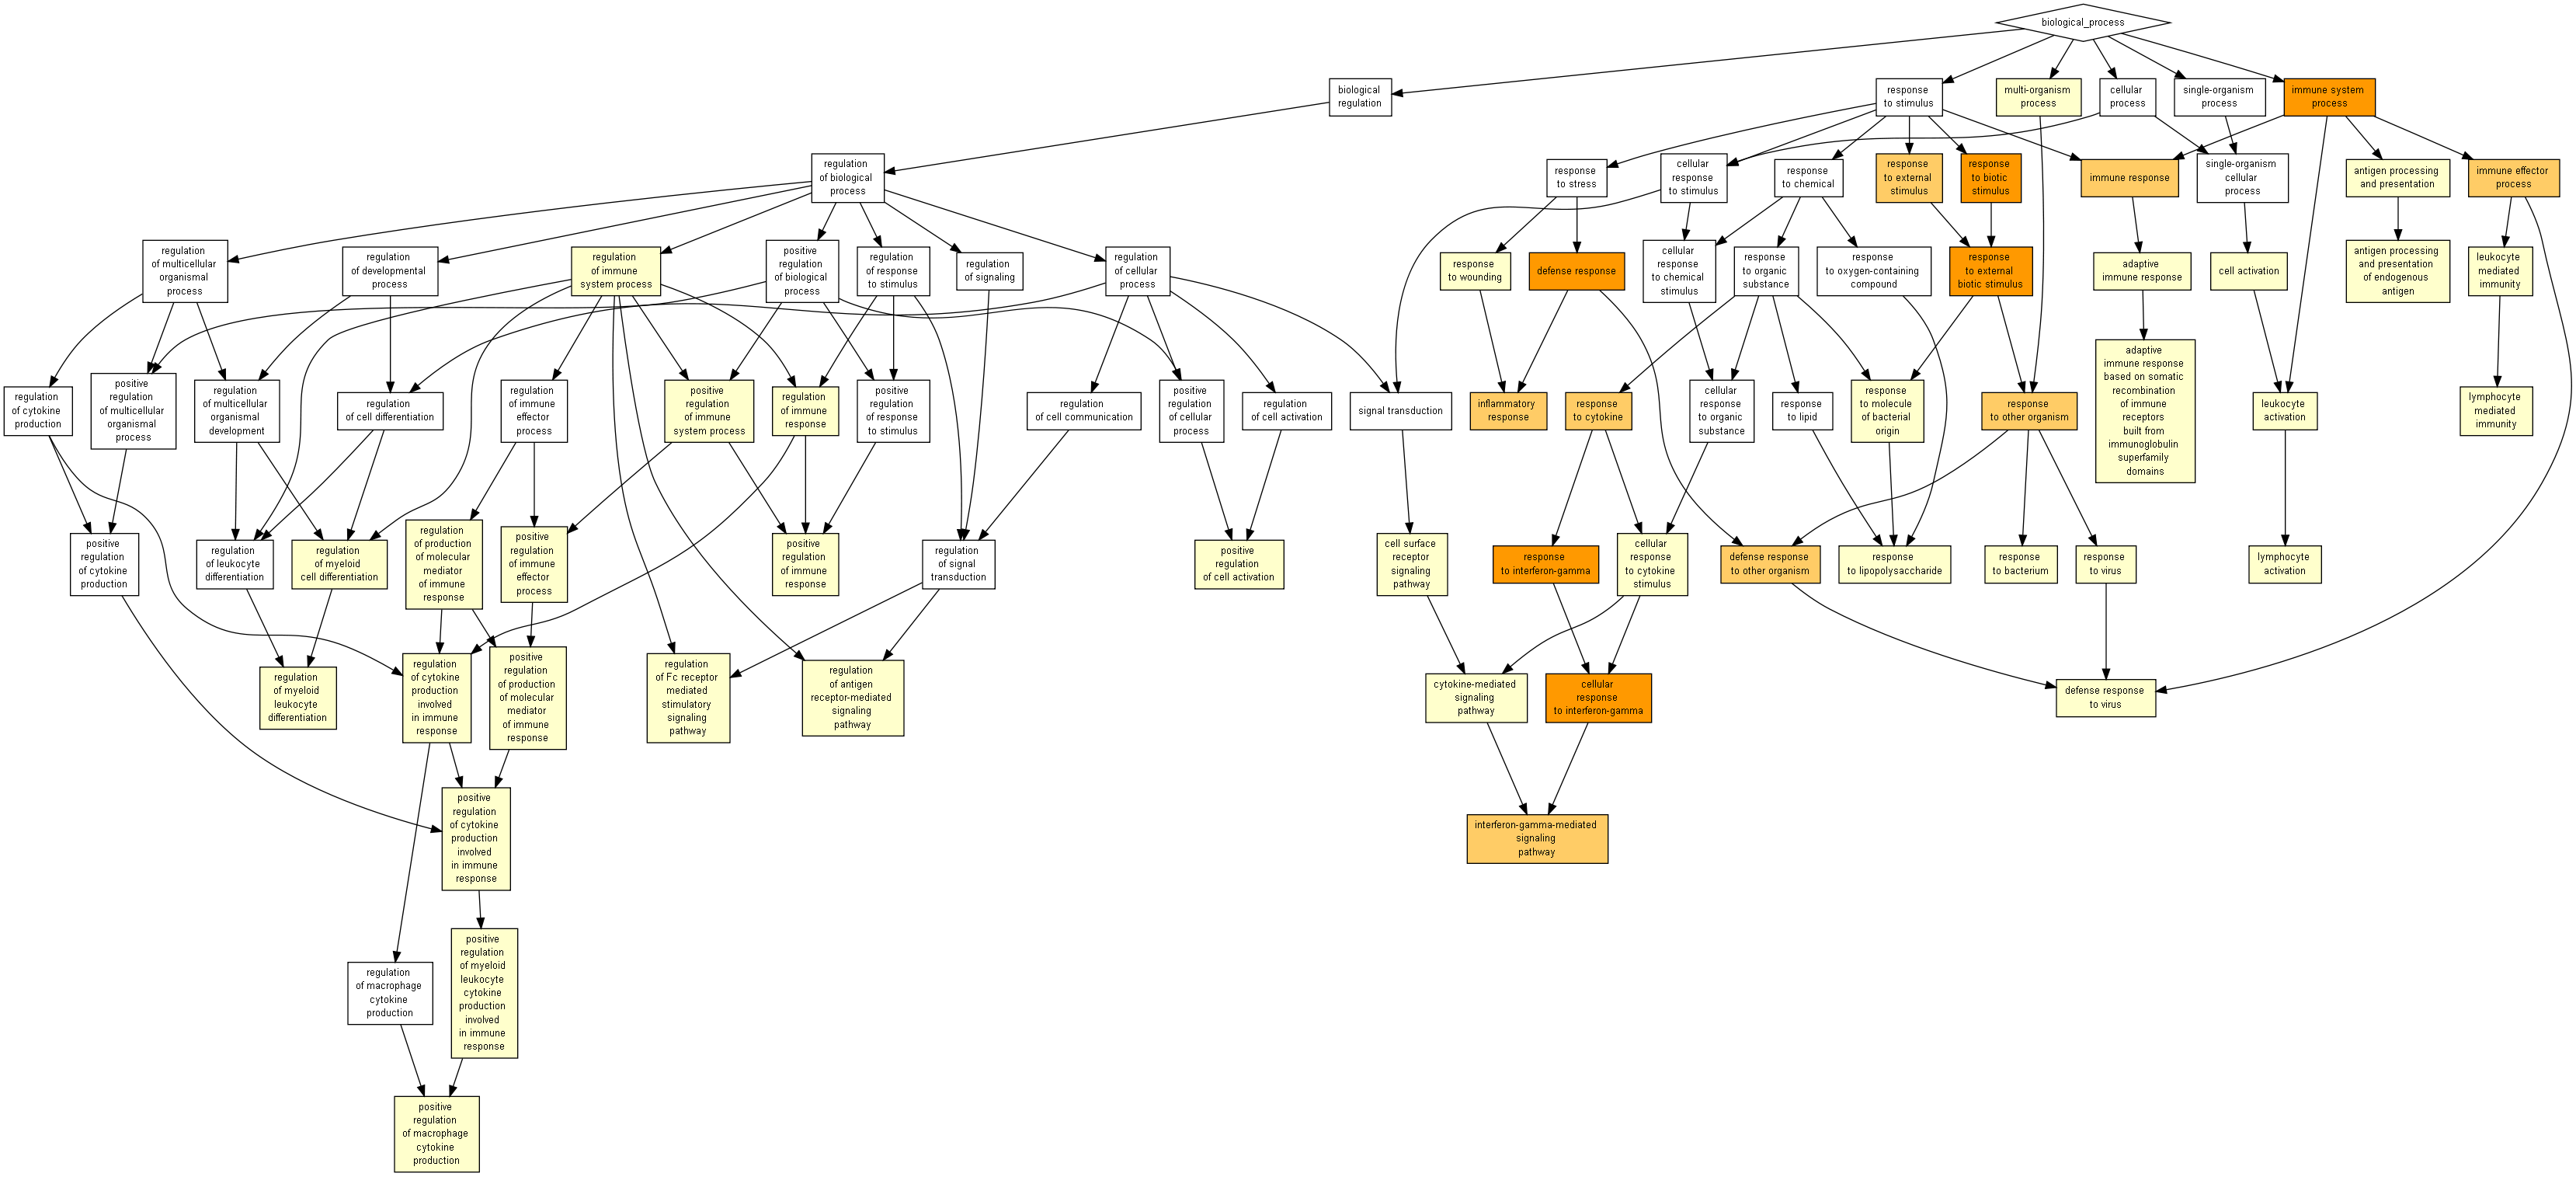
\includegraphics[width=\textwidth]
{Figures/hlc-go-pot-down/hlc-go-pot-down.png}
\caption{Vue générale}
\end{subfigure}
\end{sidewaysfigure}

\begin{figure}[p]
\ContinuedFloat
\begin{subfigure}{\textwidth}
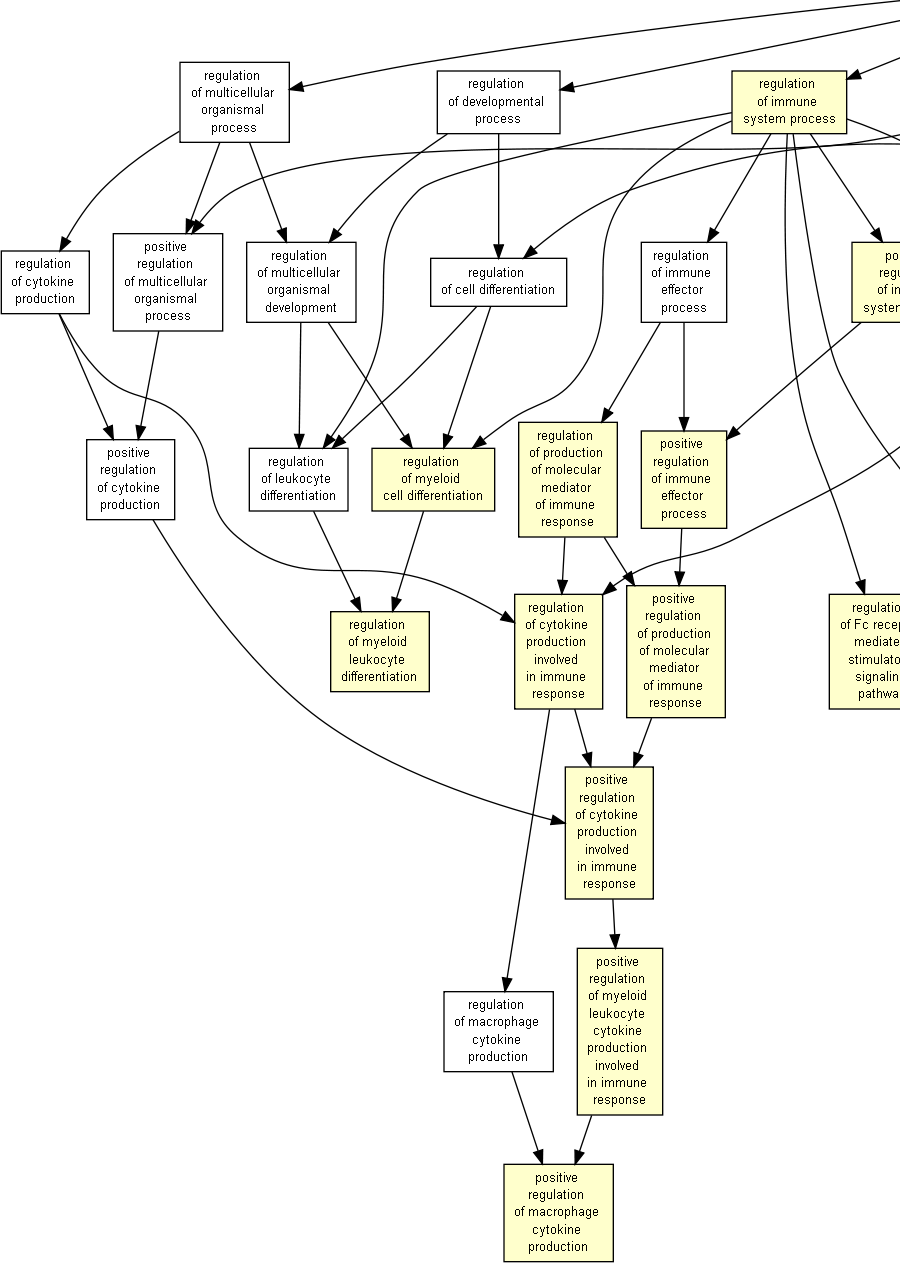
\includegraphics[width=\textwidth]
{Figures/hlc-go-pot-down/hlc-go-pot-down_0.png}
\caption{1/4}
\end{subfigure}
\end{figure}

\begin{figure}[p]
\ContinuedFloat
\begin{subfigure}{\textwidth}
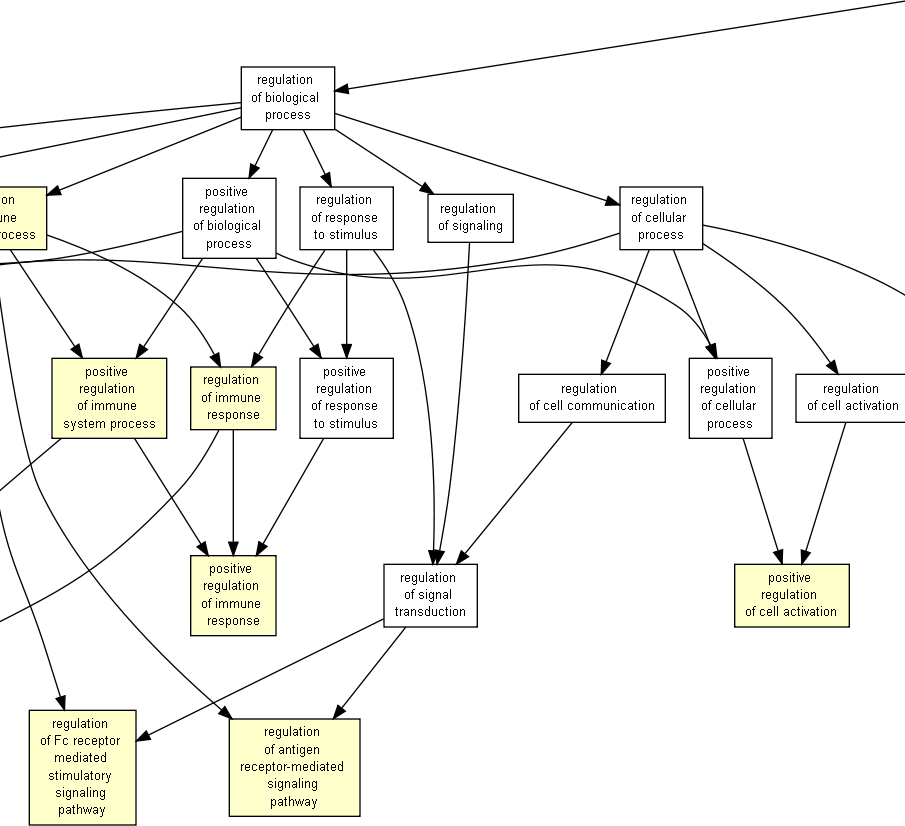
\includegraphics[width=\textwidth]
{Figures/hlc-go-pot-down/hlc-go-pot-down_1.png}
\caption{2/4}
\end{subfigure}
\end{figure}

\begin{figure}[p]
\ContinuedFloat
\begin{subfigure}{\textwidth}
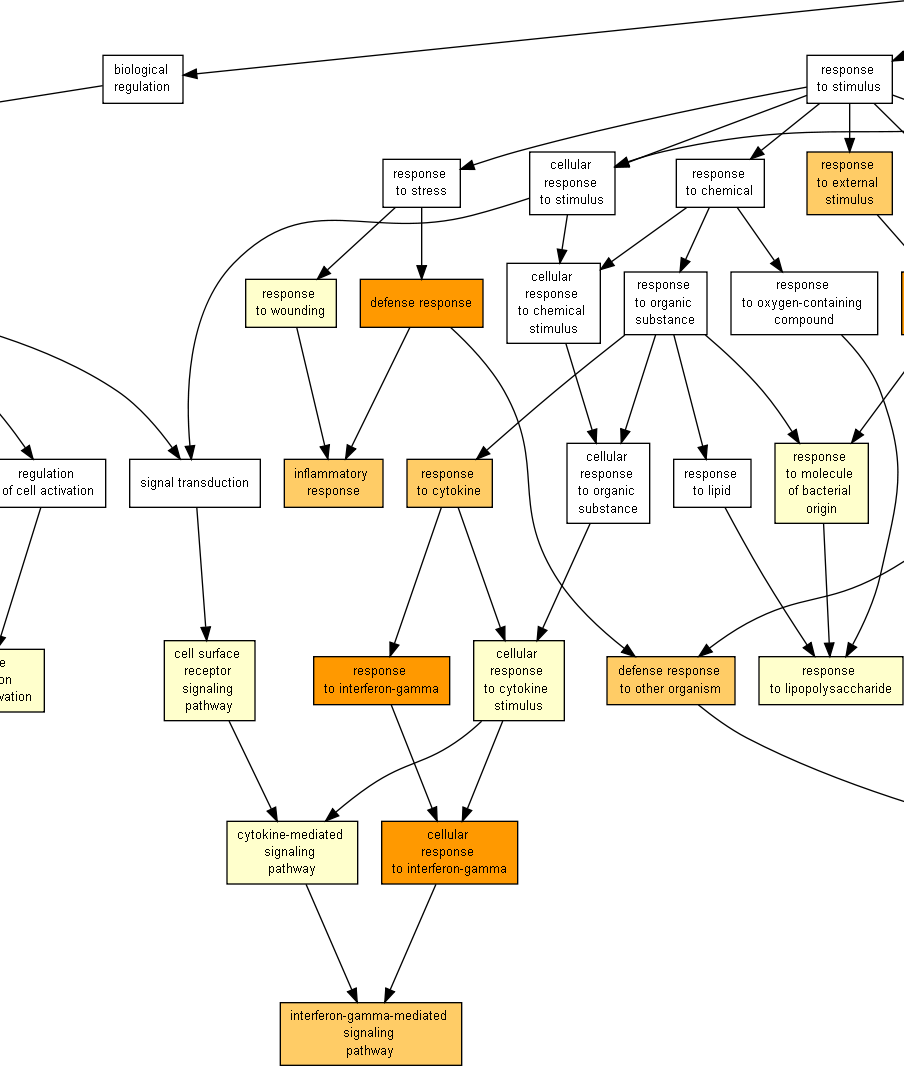
\includegraphics[width=\textwidth]
{Figures/hlc-go-pot-down/hlc-go-pot-down_2.png}
\caption{3/4}
\end{subfigure}
\end{figure}

\begin{figure}[!htp]
\ContinuedFloat
\begin{subfigure}{\textwidth}
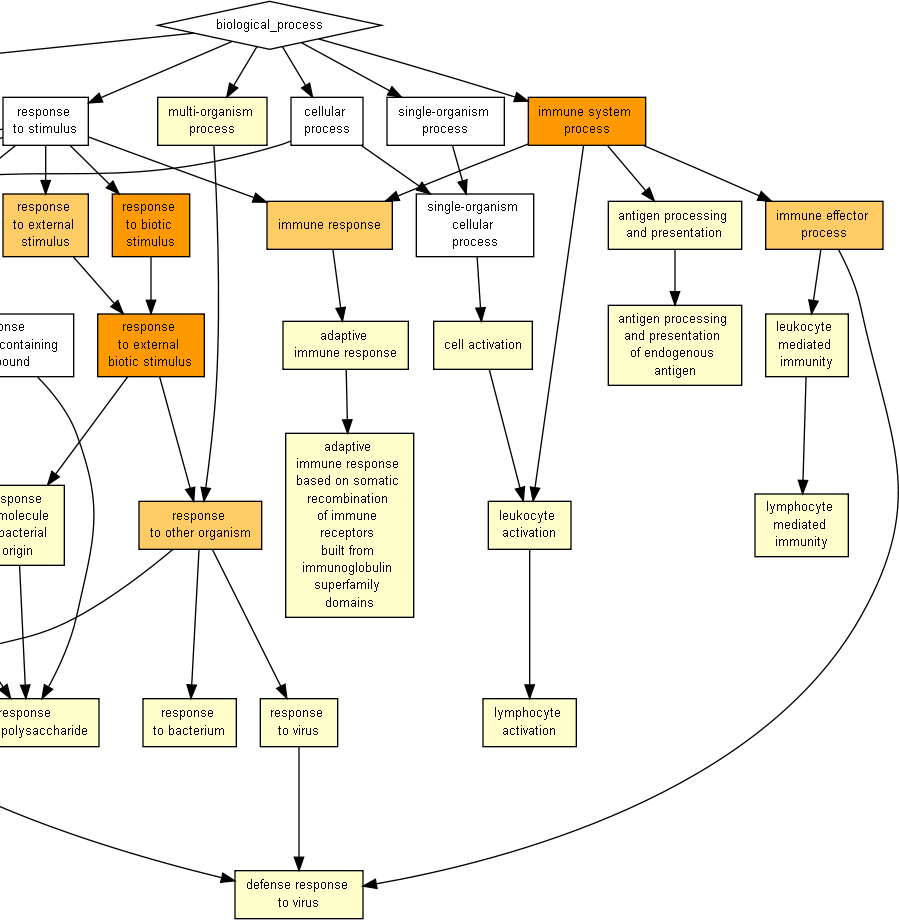
\includegraphics[width=\textwidth]
{Figures/hlc-go-pot-down/hlc-go-pot-down_3.png}
\caption{4/4}
\end{subfigure}
\caption[Enrichissement fonctionnel des gènes dont la répression \gls{t3}-dépendante est potentiée par la \gls{cort}]
{
(Cinq pages précédentes) Enrichissement fonctionnel des gènes dont la répression \gls{t3}-dépendante est potentiée par la \gls{cort}
a) Vue générale
b) Détail
L'enrichissement des termes comparé à l'ensemble des gènes transcrits est calculé à l'aide de GOrilla \citep{Eden2009}.
Les couleurs des boites correspondent à la significativité de l'enrichissement.
Jaune pâle : $10^{-5} \leq p < 10^{-3}$
Jaune : $10^{-7} \leq p < 10^{-5}$
Orange : $10^{-9} \leq p < 10^{-7}$
Rouge: $p < 10^{-9}$
}
\label{fig:hlc-go-pot-down}
\end{figure}

				Parmi les gènes participant à la sur-représentation du système immunitaire, nous trouvons notamment les orthologues de \gls{irf7}, \gls{vcam1}, \gls{cd40} ou encore \gls{ncf1}, et de plusieurs composants du \gls{mhc}, tous participant à la réponse immunitaire innée et l'activation des macrophages.


\section{Curation manuelle des termes}
	L'analyse automatique réalisée ci-dessus n'a pas permis de mettre en évidence de termes GO particulièrement enrichis, pour chacun des types de profil d'expression (excepté pour les gènes réprimés et dont l'effet des \glspl{ht} est potentié par les \glspl{gc}).
	De plus, j'ai pu observer un enrichissement, modéré à fort, de termes généraux liés au système immunitaire. Par conséquent, j'ai complété cette analyse par une recherche manuelle des termes fonctionnels comme décrit \autoref{subsec:manual-annot}
	\par
	Les résultats sont représentés sous forme d'un double histogramme vertical à deux composantes qui permet de comparer visuellement l'enrichissement des termes fonctionnels de deux groupes de gènes.
	Chaque barre est d'autant plus longue (vers la droite où la gauche) que les termes correspondants sont retrouvés dans l'une ou l'autre des listes de gènes.
	De plus, un calcul simple ($\frac{N_{i}}{\sum_{i}N_{i}}$ avec $N_i$=nombre de gènes dans le groupe $i$) permet d'estimer la répartition du nombre de gène entre les deux groupes.
	Ce dernier est représenté par un trait rouge. Par conséquent, toute déviation par rapport à la ligne rouge illustre un enrichissement ou une déplétion dans le terme correspondant.
	\par
	Cette représentation (\autoref{fig:hlc-manualannot-pot-vs-antago}) apporte quelques points à l'analyse de la Figure 3A de l'article :
	\begin{itemize} 
		\item
			Le terme lié aux maladies auto-immunes ("autoimmune") sont enrichis pour les gènes ``potentiés'' et absents des gènes ``antagonisés''. 
		\item
			Les termes liés aux pathologies osseuses sont eux aussi contrastés :
			les termes liés à la poly-arthrite rhumatoïde (``rhumatoid arthritis'') est enrichi dans les gènes ``potentiés'' et sous-représentés dans les gènes ``antagonisés''.
			Le terme ostéoarthrite (``osteoarthritis'') suit une tendance inverse.
		\item
			Les termes liés à la physiologie de l'os (``bone'', ``cartilage'', ``joints'') sont légèrement sur-représentés dans les gènes ``antagonisés''.
	\end{itemize}
	
	% BOTTOM caption
% ------------------------
\begin{figure}[!htbp]
\centering
\vspace{1\baselineskip}
\includegraphics[width=\textwidth]
% ------------------------
%
% SIDE caption
% ------------------------
%\begin{SCfigure}[\sidecaptionrelwidth][!htbp]
%\centering
%\vspace{1\baselineskip}
%\includegraphics[width=0.5\textwidth]
% ------------------------
%
% Main information
% ===========================================================
{Figures/hlc-manualannot-pot-vs-antago/hlc-manualannot-pot-vs-antago.png}
\caption[Termes enrichis dans les catégories de "potentiation" et d'"antagonisme" dans les bourgeons de membres postérieurs]
{
Termes enrichis dans les catégories de gènes "antagonisés" (valeurs négatives à gauche) et "potentiés" (valeurs positives à droite) dans les \glspl{hlb}.
La valeur absolue de l'axe des abscisses représente le nombre de gène associé à chaque terme (axe des ordonnées).
Seuls les 50 termes les plus représenté sont illustrés ici.
Les barres verticales rouge correspondent au nombre théorique de gènes associés à chaque terme dans le cas d'une répartition aléatoire entre profils "antagonisés" et "potentiés".
Les termes bleus sont associés au squelette.
}
\label{fig:hlc-manualannot-pot-vs-antago}
% ===========================================================
%
% BOTTOM caption
% ------------------------
\end{figure}
% ------------------------
%
% SIDE caption
% ------------------------
%\end{SCfigure}
% ------------------------

	Pour analyser plus finement les fonctions biologiques associées aux profils ``d'antagonisme'', j'ai représenté sous forme de double-histogramme vertical les effectifs des gènes réprimés (à gauche) ou induits (à droite) associés à différentes fonctions biologiques (\autoref{fig:hlc-manualannot-antago}).
	Il y a une asymétrie forte pour les gènes associés à l'ostéoarthrite.
	Il sont en effet enrichis en gènes dont l'induction \gls{t3}-dépendante est antagonisée par la \gls{cort}

	% BOTTOM caption
% ------------------------
\begin{figure}[!htbp]
\centering
\vspace{1\baselineskip}
% ------------------------
%
% Main information
% ===========================================================
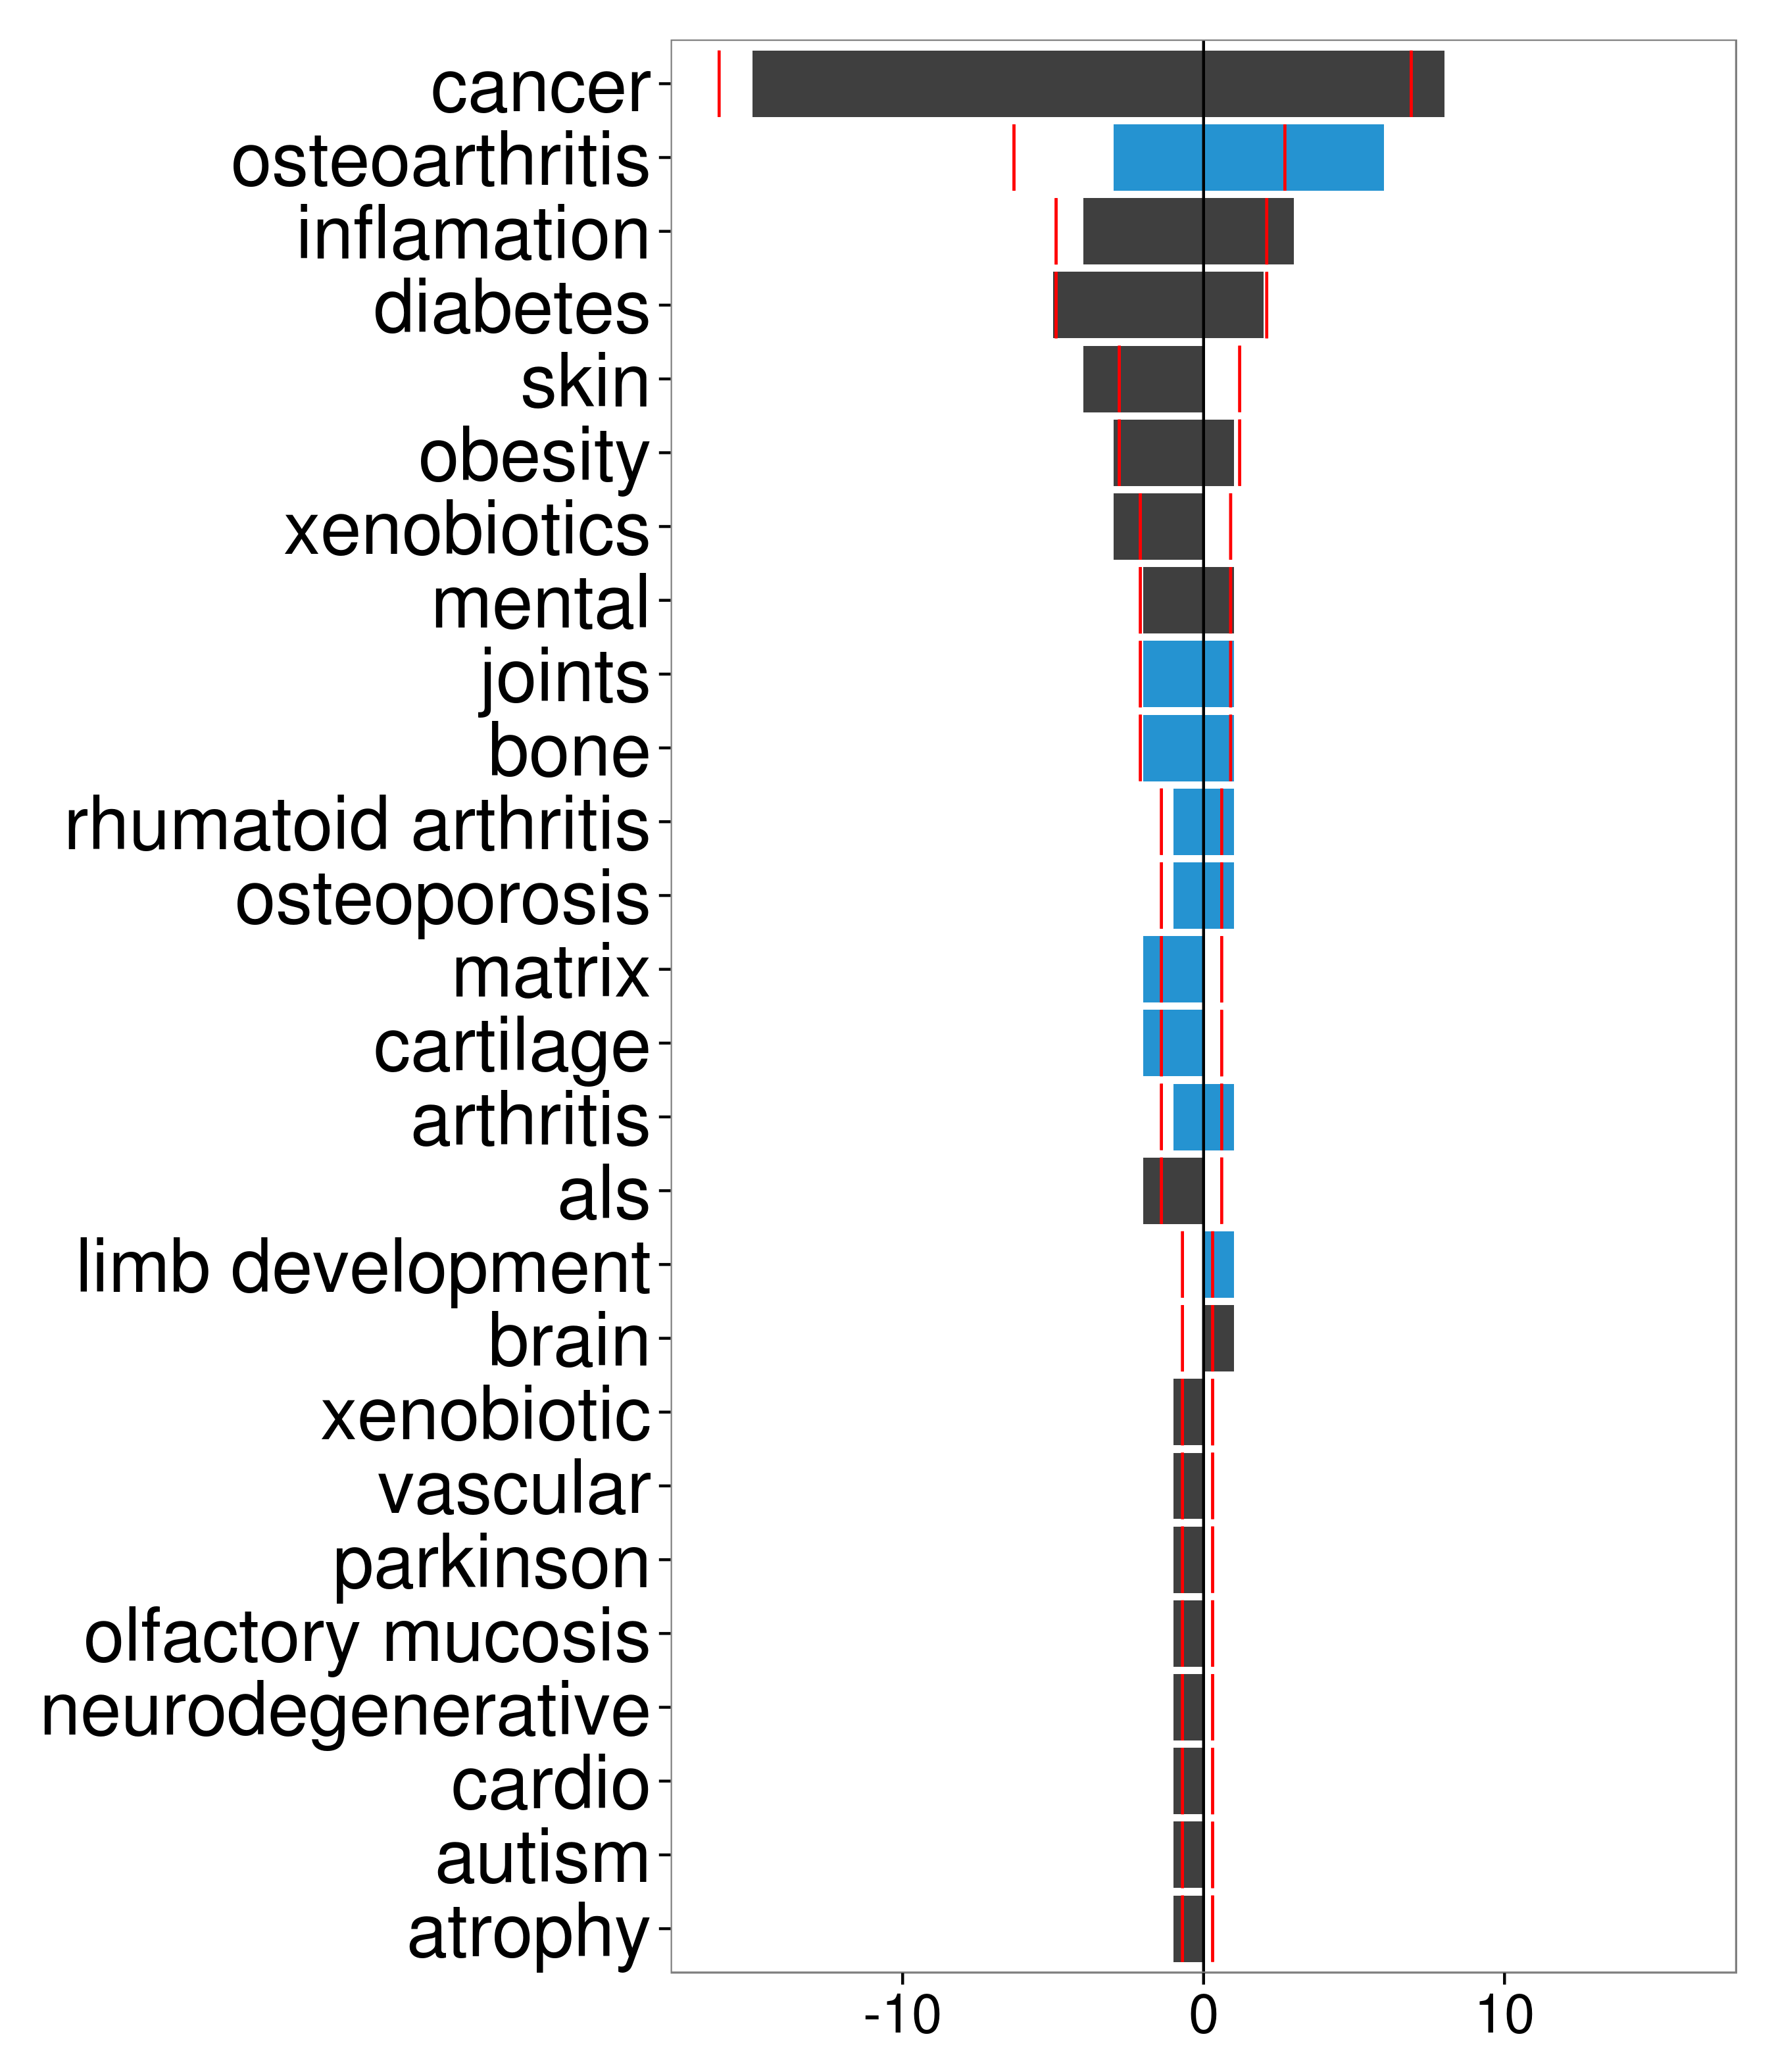
\includegraphics[width=0.8\textwidth]
{Figures/hlc-manualannot-antago/hlc-manualannot-antago.png}
\caption[Catégories fonctionnelles enrichies parmi les gènes ``antagonisés'' dans les bourgeons de membres postérieurs]
{
Catégories fonctionnelles enrichies parmi les gènes présentant un profil d'``antagonisme'' et réprimés (valeurs négatives, partie gauche) ou induits (valeurs positives, partie droite) dans les \glspl{hlb}.
La valeur absolue de l'axe des abscisses représente le nombre de gène associé à chaque terme (axe des ordonnées).
Les barres verticales rouge correspondent au nombre théorique de gènes associés à chaque terme dans le cas d'une répartition aléatoire entre répression et induction.
Les termes bleus sont associés au squelette.
}
\label{fig:hlc-manualannot-antago}
% ===========================================================
%
% BOTTOM caption
% ------------------------
\end{figure}
% ------------------------

	L'analyse des gènes ``potentiés'' révèle une situation contrastée \autoref{fig:hlc-manualannot-pot} pour les termes liés à l'inflammation (``inflammation''), peau (``skin'') et le système vasculaire (``vascular''). 

	% BOTTOM caption
% ------------------------
\begin{figure}[!htbp]
\centering
\vspace{1\baselineskip}
\includegraphics[width=\textwidth]
% ------------------------
%
% SIDE caption
% ------------------------
%\begin{SCfigure}[\sidecaptionrelwidth][!htbp]
%\centering
%\vspace{1\baselineskip}
%\includegraphics[width=0.5\textwidth]
% ------------------------
%
% Main information
% ===========================================================
{Figures/hlc-manualannot-pot/hlc-manualannot-pot.png}
\caption[Termes enrichis dans les catégories de "potentiation" dans les bourgeons de membres postérieurs]
{
Termes enrichis dans les catégories de "potentiation" entre les effets des deux hormones dans les \glspl{hlb}.
Les valeurs négatives (partie gauche) correspondent à une potentiation de l'effet répresseur des hormones.
Les valeurs positives (partie droite) correspondent à une potentiation de l'effet inducteur des hormones.
La valeur absolue de l'axe des abscisses représente le nombre de gène associé à chaque terme (axe des ordonnées).
Les barres verticales rouges correspondent au nombre théorique de gènes associés à chaque terme dans le cas d'une répartition aléatoire entre répression et induction.
Les termes bleus sont associés au squelette.
}
\label{fig:hlc-manualannot-pot}
% ===========================================================
%
% BOTTOM caption
% ------------------------
\end{figure}
% ------------------------
%
% SIDE caption
% ------------------------
%\end{SCfigure}
% ------------------------

\end{document}